% latexmk -pvc -pdf
\documentclass[a4paper]{article}
\usepackage[margin=0.65in]{geometry}
\usepackage{multicol}
\usepackage{amsthm,amsfonts,amssymb}
\usepackage[english]{babel}
\usepackage{blindtext}
\usepackage{sidecap}
\usepackage{caption}
\usepackage{subfig}
\usepackage{graphicx}
\newenvironment{Figure}
    {\par\medskip\noindent\minipage{\linewidth}}
    {\endminipage\par\medskip}

\title{
    
}
\author{Ana C. Fabela Hinojosa \\
\small{School of Physics and Astronomy, Monash University}}
\date{Last edit: \today}

\begin{document}
\maketitle

\begin{abstract}
We investigate how the range (distance travelled) by alpha particles changes as the alpha particles interact with a surrounding medium. The experiment aims to describe the observed energy spectrum for alpha particles emitted from a radioactive \textsuperscript{241}Am source. By increasing air pressure in a sealed vacuum chamber we are able to determine the straggling parameter as the emitted particles travel through the chamber into a detector -------. In this investigation we also calculate the thickness of the gold overcoat layer of the radioactive source ------- and we compare it to the manufacture value ------.

\end{abstract}

\section{Introduction}
\begin{multicols}{2}

The least penetrating type of ionizing radiation consists of two protons and two neutrons (nucleons) bound together in alpha particles.\cite{SPA, alpha}

When an atom's nucleus emits an alpha particle, the atom's mass number decreases by four due to the loss of the four nucleons that make the alpha particle\cite{alpha}. 
In this type of decay event, the created alpha particle and daughter nucleus must balance out the strong force (given the nuclear scale) with newly aquired coulomb repulsion (both the daughter nucleus and alpha particle have net positive electric charges). The apha particle is eventually be ejected form the nucleus.

Because of it's net positive charge, the ejected alpha particle will interact by means of the coulomb force with the surrounding medium. Which will lead to a kinetic energy loss.\cite{SPA}

As the alpha particle moves through matter, it ionizes and thus loses kinetic energy in many steps, until it's energy approaches zero. The travelled distance is called the range of the particle.\cite{straggling}.
\subsection{Detection of alpha particles}
When an incident charged particle enters the detector, electron-hole pairs are created as the particle is descelerated. The charges are drawn to the appropriatesurface contact, crating a charge pulse that is proportional to the energy of the charged particle.\cite{SPA}
We use a pulse amplifier to convert charge-to-voltage, providing us an output voltage that is proportional to the charge produced by the input photo diode\cite{SPA}
We then, detect the voltage pulses with the multichannel analyser, and record the pulses heightsin a series of internal bins producing a histogram of pulses heights.\cite{SPA}

\section{Background Theory}
 Alpha particles do not have enough kinetic energy to escape the potential well from the strong force inside the nucleus. Nevertheless, due to quantum tunnelling and the coulomb repulsion effect the created alpha particles spend some time in a region so far from the nucleus that the potential from the repulsive electromagnetic force has fully compensated for the attraction of the nuclear force\cite{alpha}. 
Causing the ejection of the particle from the nuclear region.  
 
\subsection{The decay path of \textsuperscript{241}Am}
The most probable alpha decay event occurs with $85\%$ probability.
The mean life of \textsuperscript{241}Am is 458 years.\cite{SPA}
An \textsuperscript{241}Am nucleus decays to a \textsuperscript{237}Ne, a \textsuperscript{4}He nuclei and a gamma ray with $E = 59.6$ keV\cite{americium}
\subsection{The range of \textsuperscript{241}Am}
In 1933 Hans Bethe developed the Bethe formula which describes the mean energy loss per distance travelled by charged particles\cite{Bethe}

\begin{equation} \frac{-\mathrm{d} E}{\mathrm{d} x} = B \rho E_0^{- 0.73}
\end{equation}

where $B = 2.58$ MeV (cm kg m\textsuperscript{-3})\textsuperscript{-1}, $E_0$ is the initial kinetic energy of the alpha particle, the density of air at $20^{\circ}$C and $101.325$kPa: $\rho = 1.204$kgm\textsuperscript{-3} and finally x is the distance travelled by the particle in cm.

We integrate equation (1) with respect to distance to obtain the range of the alpha particles as a function of initial energy
\begin{equation} R = \frac{E_0^{1.73}}{1.73 B \rho}
\end{equation}
From this we can calculate a theoretical expression for the range at one atmosphere.\cite{SPA}
\begin{equation} R_{atm} = 0.186 E_0^{1.73}
\end{equation}

Since energy loss is proportional to the number of gas molecules encountered\cite{SPA}, we use 
\begin{equation} R = R_{atm} \frac{P_{atm}}{P},
\end{equation}
where $P$ is the pressure and $P_{atm}$ is the atmospheric pressure, assuming that air behaves as an ideal gas this implies that the density of air molecules will vary linearly with the pressure P \cite{SPA} as per the following expression
\begin{equation} \rho = \frac{P}{R_d T},
\end{equation}
where T is the absolute temperature of the gas and $R_d = 287.05$J(kg K)\textsuperscript{-1} is the specific gas constant.
Using this relation the range R becomes:
\begin{equation} R = 64.31 \frac{T}{p} E_0^{1.73},
\end{equation}
where the energy is measured in MeV \cite{SPA}. 

\subsection{Range straggling}
All alpha particles have the same initial mass-energy. It's likely that the reader might assume that if the emitted alpha particles interact with a homogeneous medium their ranges should be identical.

Nevertheless, experiments show that random variations in the effective path lengths occur due to the molecular nature of air. Which leads us to consider the statistical nature of such interactions. The number of collisions required to bring an alpha particle to rest within the medium will vary slightly, depending on the number of collisions the particle suffers.
Hence, there will be a small variation in the particle's range. This is known as straggling. \cite{straggling}

It is also important to mention why the approach of varying the pressure in the chamber is used instead of modifying the distance between the source and the detector.
Both approaches are theoretically identical but for practical purposes a fixed chamber size is used. Another geometric consideration is that modifying the distance to the detector changes the solid angle of the ejected alpha particles; changing the number detected particles independently of other loss mechanisms\cite{feedback}.

To determine the full straggling parameter $(\alpha)$, we must consider an additional dispersion in the energy spectrum, which occurs due to the construction of the radioactive source used in this experiment. 
The source has a layer of gold that covers the surface where the radioactive source rests $\alpha_{source}^2$\cite{SPA}. 

Thus we write our expression for the straggling parameter as the sum
\begin{equation} \alpha^2 = \alpha_{air}^2 + \alpha_{source}^2,
\end{equation}

where the straggling parameter of alpha particles in air $(\alpha_{air})$ is characterised by 
\begin{equation} \alpha_{air} = 0.6006 FWHM,
\end{equation}
where FWHM is the 'full width half maximum' of the distribution of the energy spectrum. 

We examine the number of alpha particles as the pressure chamber is varied
\begin{equation} n(p) = \frac{n_0}{2} \left (1- erf \left (\frac{p - p_0}{\alpha}\right )\right ),
\end{equation}
where p is the varying air pressure in the chamber, $n_0$  is a large number of particles with initial velocity $(v_0)$ (this parameter will be useful for normalisation), $p_0$ is the pressure preventing alpha particles from reaching the spatially fixed detector ($x_0$ cm away from the radioactive source) and $\alpha$ is the full straggling parameter we defined earlier.

\subsection{Bragg--Kleeman rule}
As we described in section 2.3 in order to determine the correct straggling parameter in our experiment we must correct for the construction of the radioactive source. The effective stopping power of materials other than air is approximately inversely proportional to $\rho$ the density and $\sqrt{A}$ where $A$ is the atomic mass of the substance through which the alpha particle travels.

The Bragg--Kleeman rule is used to predict the energy loss for alpha particles passing through a material by comparing it to a reference material
\begin{equation} \frac{R_1}{R_0} = \frac{\rho_0}{\rho_1}\sqrt{\frac{A_1}{A_0}},
\end{equation}

where $R_0$is the range of the alpha particles in the reference material and $R_1$ is the range of the alpha particles in the new material.

In this experiment the reference material used is air.
in the experimental script we are previded with the values for $\sqrt{A_0} = \sqrt{A_{air}} = 3.82$ and $\rho_0 = 1.204$kgm\textsuperscript{-3}. We calculated the $R_0 = R_{atm}$ in equation (3).

We use equation (9) to find the range of alpha particles travelling through gold given the layered construction of our radioactive source. We require an expression to predict the energy loss from alpha particles travelling through the gold layers of the construction(a distance $\Delta x$). 
From integrating equation (1) we obtain
\begin{equation} E = \left(E_0^{1.73} -0.0156 \rho \frac{\Delta x}{T} \right)^{0.578},
\end{equation}
here we can use equation 9 and replace $\rho =  \rho_1\sqrt{\frac{A_{air}}{A_1}}$
\begin{equation} \therefore E = \left(E_0^{1.73} -0.0156 \rho_1\sqrt{\frac{A_{air}}{A_1}} \frac{\Delta x}{T} \right)^{0.578},
\end{equation}
where $\rho_1 = \rho_{gold} = 19.30 * (g / cm^3), A_1 = A_Au = 196.966570$ are the density and atomic mass of gold\cite{gold}

\section{Method}
The experimental set up allows for the acquisition of data pulses that have pulse height greater than 10 bins for 300s in 1024 bins. 
This bin number has been chosen to optimise for an adequate signal to noise ratio as well as resolution of the spectrum.
The MCA device will only record a new pulse after the input voltage drops below the threshold level\cite{SPA}.
Below we outline the procedure followed in order to configure our experimental apparatus for optimal operation. 

\subsection{Alpha particle detection}
To configure our detector, we by turn "on" the power switch of the "NIM" bin and turning "on" the MCA and DSO amplifier units.
\subsection{Adjusting chamber pressure}
The chamber pressure is controlled by admitting air into the chamber using the "air admit" valve. If partial evacuation of the chamber is required, repeat the steps described below.
We first close the air admittance valve and proceed to turn "on" the vacuum gauge. We activate the pump and open the "Vacuum pump line". The aparatus will start removing air from the chamber, once the pressure is below $0.05$kPa we close the "Vacuum pump line" and finally we deactivate the pump. 
We proceed by ensuring that the amplifier output is connected to DSO the particle pulses are detected to be approximately $> 2$ V. Whe finally make sure amplifier output is connected to MCA unit
(Note that the threshold value might have to be readjusted).

\subsection{MCA software set-up}
In order to operate the detector we must launch "ADMCA" software. Once we start the software in the computer an initialisation menu will require us to accept default device (MCA8000A) attached to the computer and experimental apparatus. we click "connect" and proceed by adjusting the data acquisition settings.
In the MCA menu we click 'Acquisition set up' and we ensure preset mode is set to 'seconds'. After this we proceed to ensure that the timer is set to 'live time' with preset time t = 100s.
The 'threshold' is set to 42 and the 'ADC channels' to '1024'
After this configuration is set we click 'ok' to preserve this settings.
The final steps are to clear any data stored in the MCS memory by clicking in the MCA menu "Delete data and Reset time" and finally we 
click in the MCA menu the "Start acquisition" option to begin with our data acquisition.

To visualise our data, we defined a region of interest (ROI) for the software. Clicking "edit ROI" on the toolbar and dragging a cursor over the region containing the visible peak. We exit this tool by clicking "edit ROI" once again. The spectra is saved in an ASCII file format which we analysed using python.
As the pressure increases the alpha particle spectrum moves towards the lower energy region and the spectrum skews.
It is therefore necessary that we estimate the peak position manually for each spectrum. We do this by computationally finding the maximum count value and the FWHM of each of the spectra.

\subsection{Detector's Zero energy}
The experimental script informs us that the output for the detector's zero signal does not necessarily correspond to zero volts. In adition to this, the first bin of the MCA spectrum will not necessarily correspond to the zero input signal\cite{SPA}.

To find the baseline signal of the detector it is useful to fill  the  chamber  with  air  completely as this will  stop  all  alpha  particle  detection events\cite{SPA}.
The  MCA  unit’s detection range is set between 0 and 5 volts, we assume that the first and last bins in the MCA range correspond exactly to a 0 and 5 volt input respectively and we proceed to calibrate the visible x axis. 

Converting the measured voltage into an anticipated MCA bin value requires us to multiply the x-axis by the estimated size of each bin.
We therefore correct your data by considering the background count offset using the calibrated x-axis, and the threshold observed.

Another important factor for obtaining an adequate spectrum is to make sure the threshold used is set to cut out the majority of the background noise peak. Nevertheless this presents a problem since the obtained spectrum of the particles fails to be complete at low energies given the cutting out of the noise peak. We fix this issue by extrapolating the spectrum. We choose to take an average of the first 50 values above the threshold for each data set. Thus obtaining a representative curve that accounts for the shape and noise of our data. 

In order to find a representative value for the peak of each spectra we processed our data using a gaussian smoothing technique. We simply convolved the raw data with a gaussian that has $\sigma = 4$ From this it was straight forward to find an estimate for the mean of each distribution.
We calculate an uncertainty estimate for this process by observing the data and estimating the possible uncertainty in the computed mean form the smoothed data. We also calculated a rough uncertainty in the  mean count by observing the size of our noise and dividing this by the square root of the number of bins present in the FW of the gaussian used for the convolution.
The uncertainty in the bin position of the mean (peak position $\pm$ 8)is the same as the vertical uncertainty in figure 3 in the analysis.

HOW DOES THE UNCERTAINTY PROPAGATION WORK???????????????????


\begin{equation} u(\mu_{count}) = \frac{\sigma}{ \sqrt{N}},\\\therefore \frac{80}{ \sqrt{8}} \approx 30,
\end{equation}
\end{multicols}

\newpage
\section{Results}
Data acquisition parameters
\begin{itemize}
    \item Laboratory temperature $T = 294.15 \pm 0.5 K$
    \item MCA threshold $ = 42$
    \item Acquisition time $t = 100s$
    \item Background threshold: $4$
\end{itemize}

\begin{figure}[!htb]
\subfloat[]{\scalebox{0.37}{
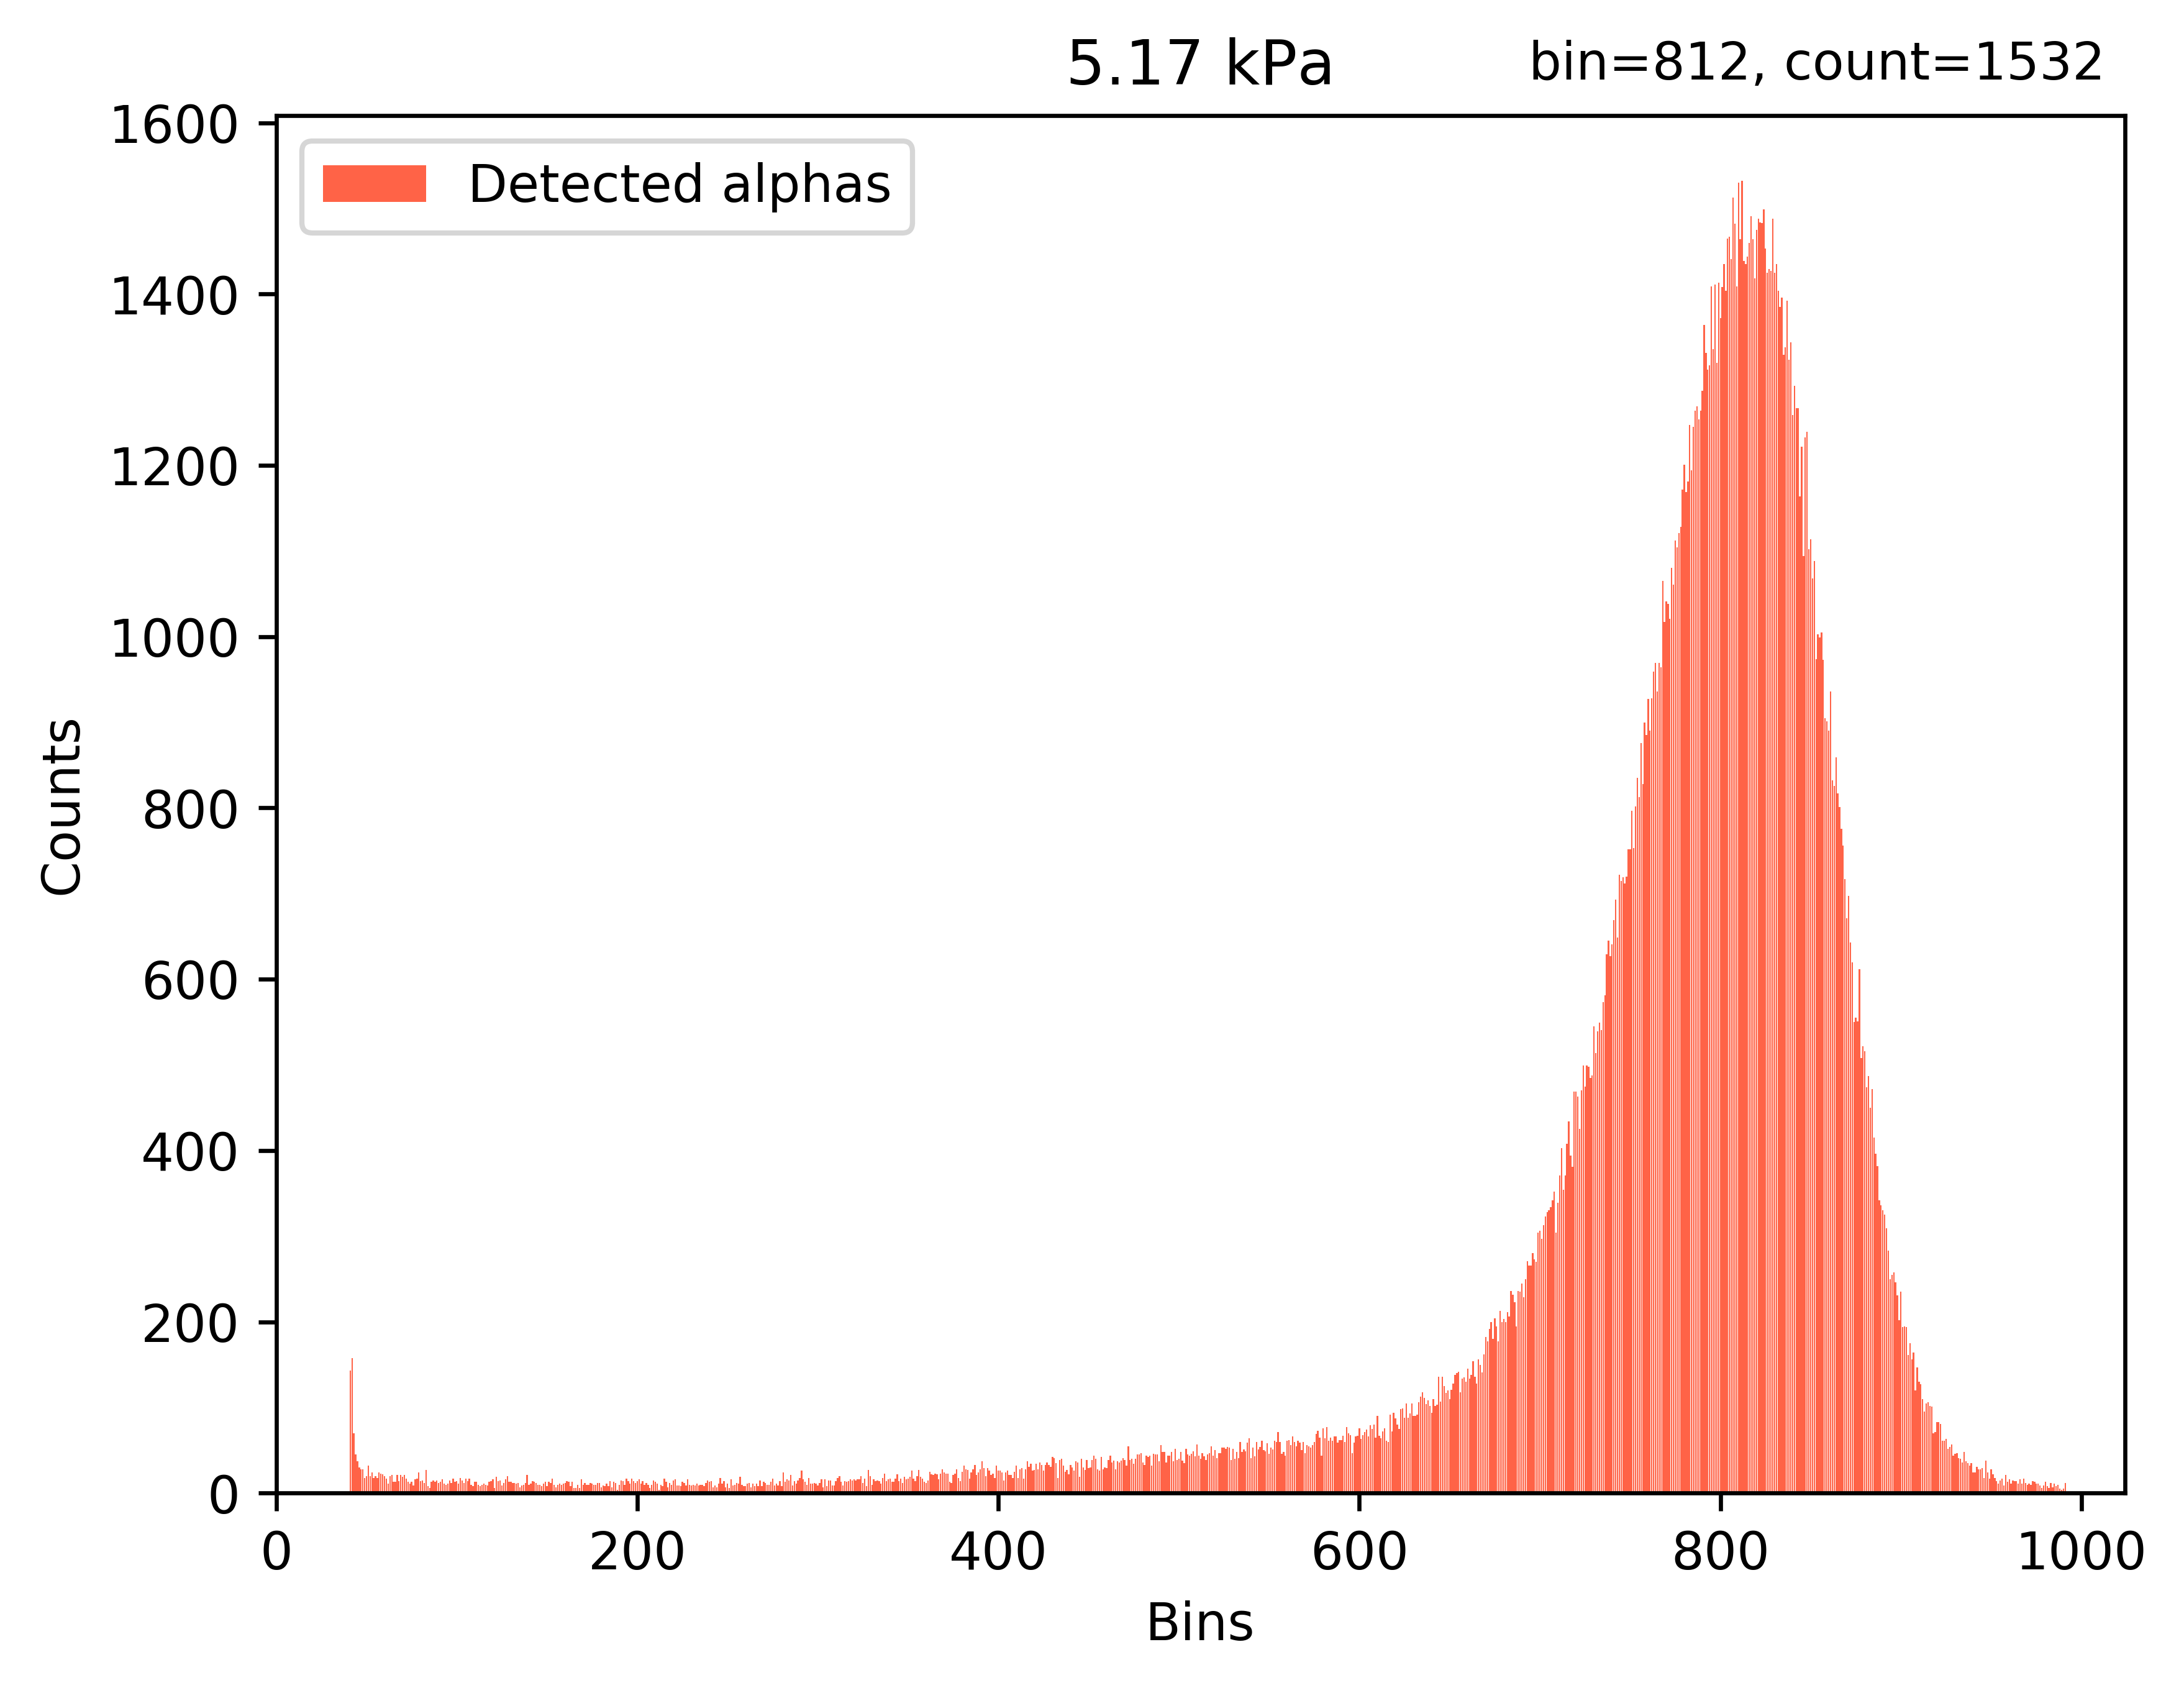
\includegraphics{raw_p=5.17kPa.png}    
}}
\subfloat[]{\scalebox{0.37}{
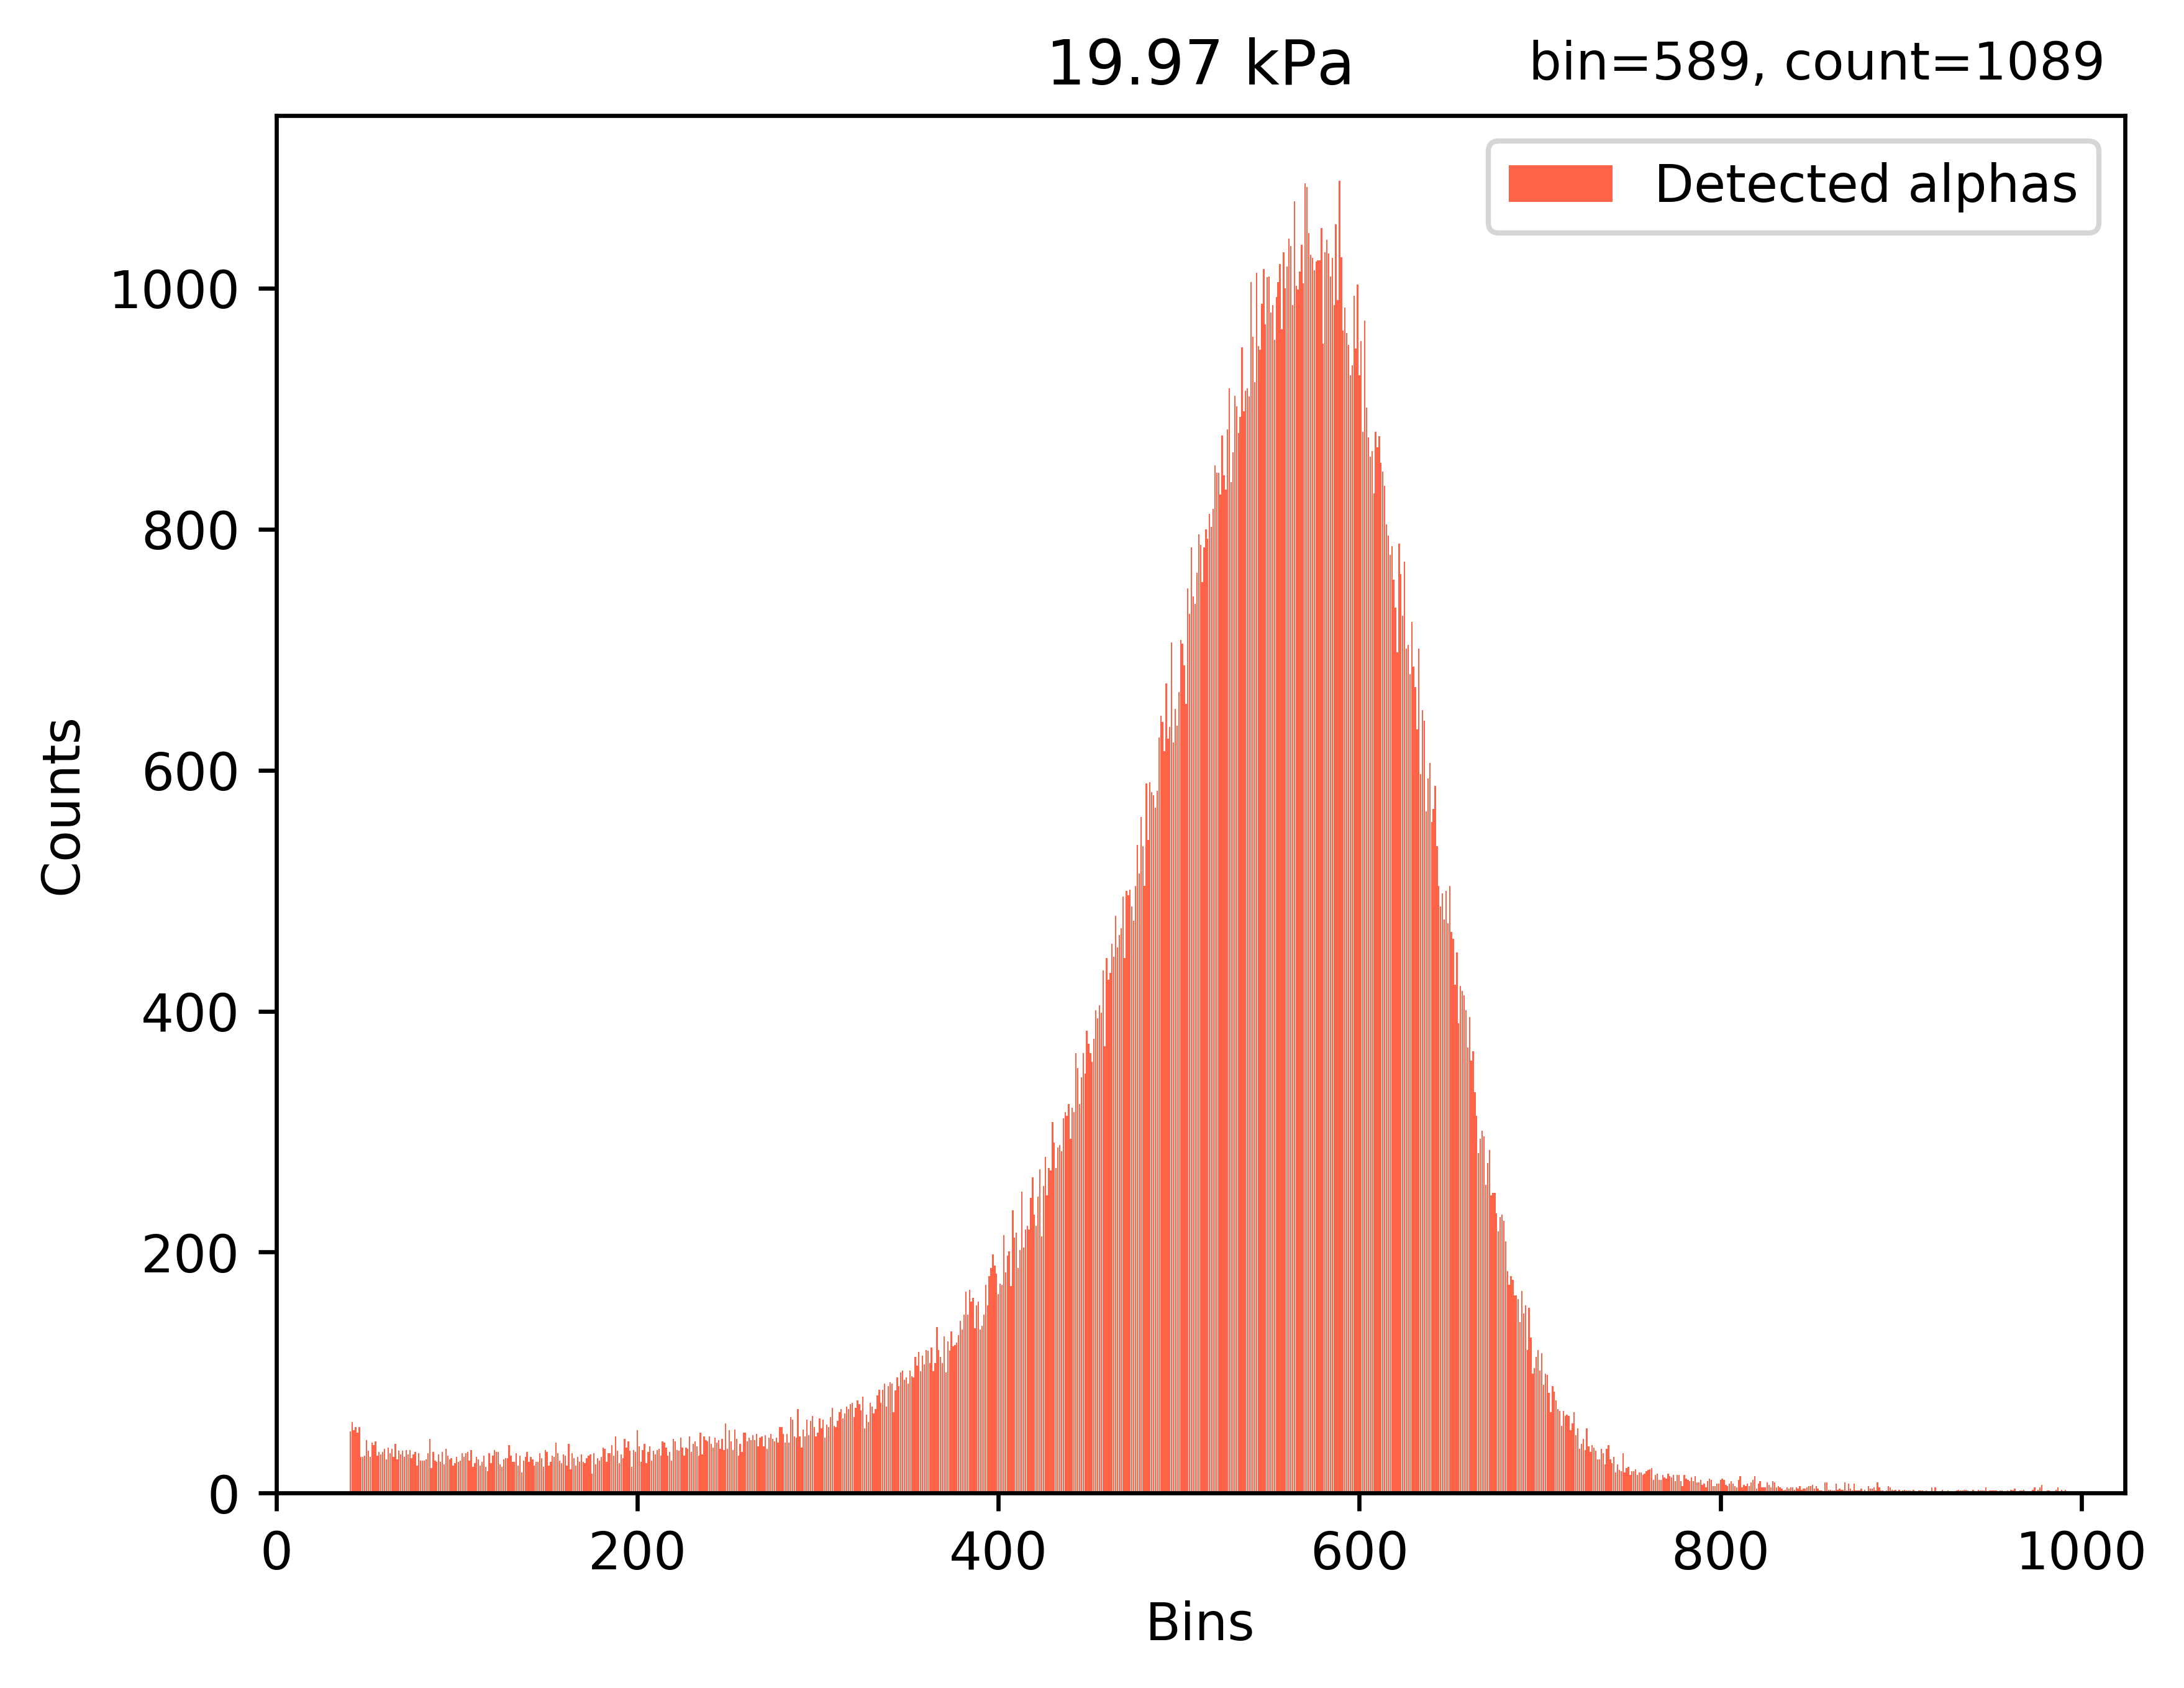
\includegraphics{raw_p=19.97kPa.png}   
}}
\subfloat[]{\scalebox{0.37}{
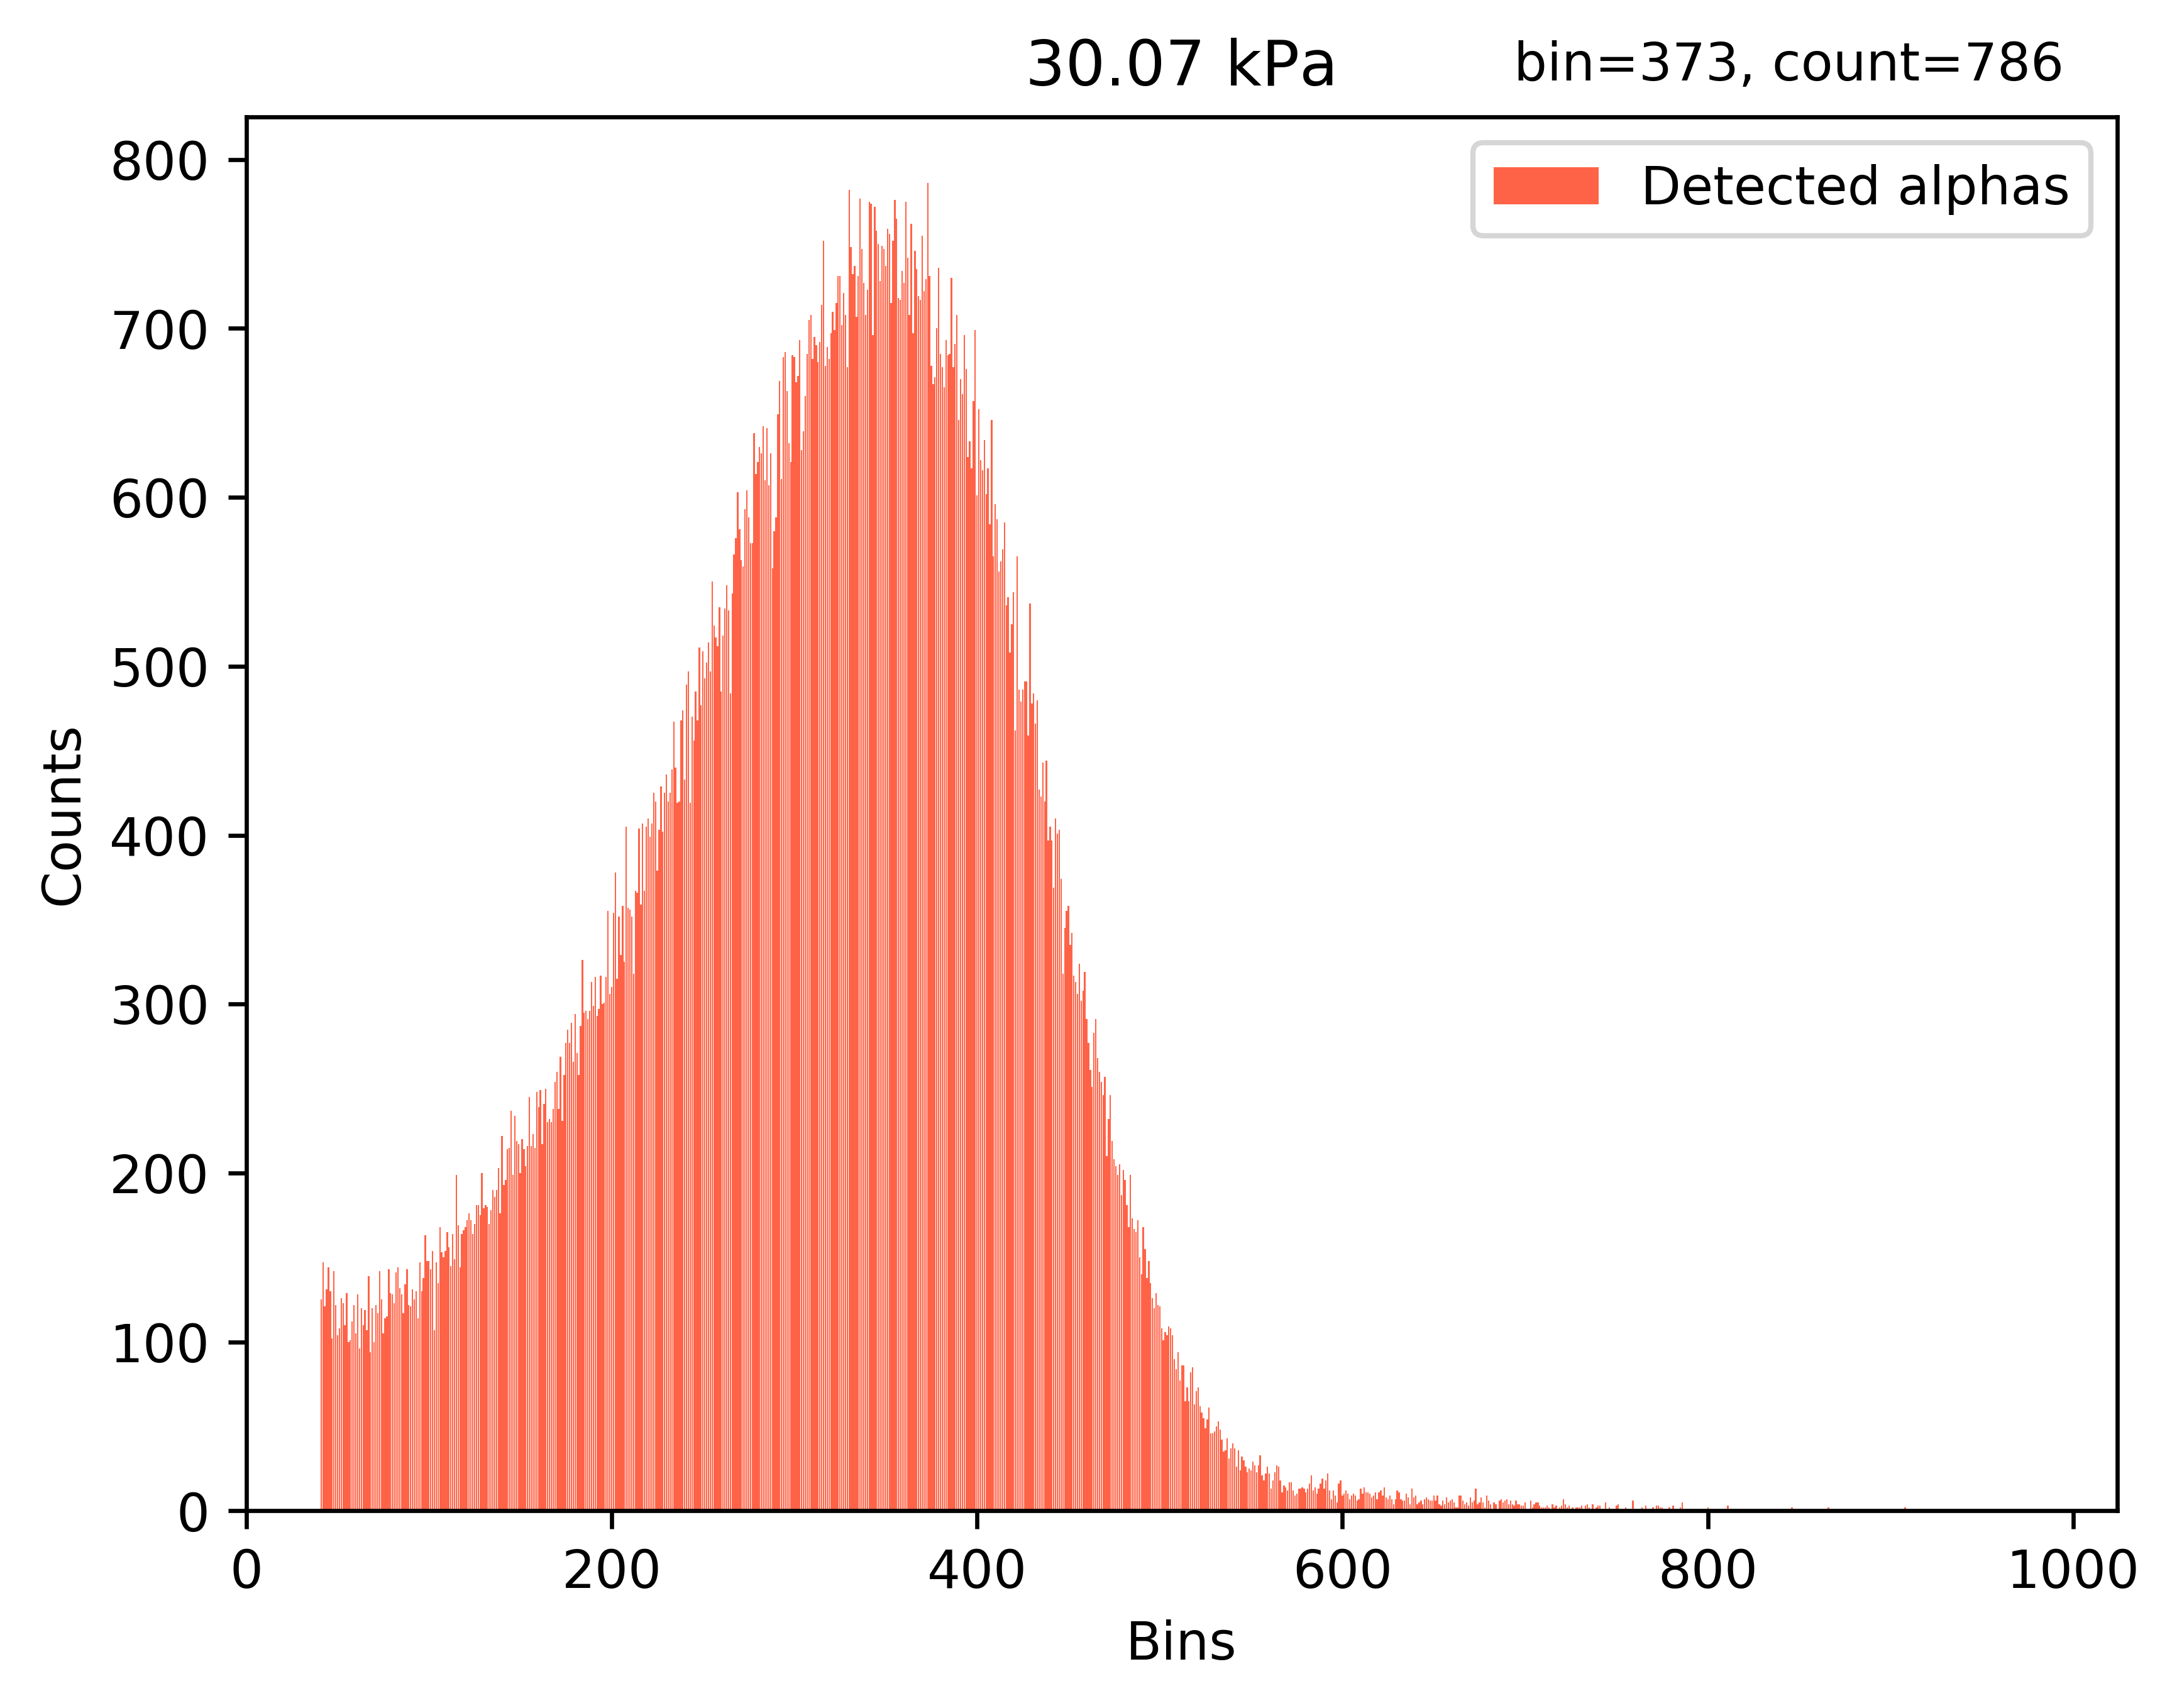
\includegraphics{raw_p=30.07kPa.png}
}}\\
\subfloat[]{\scalebox{0.37}{
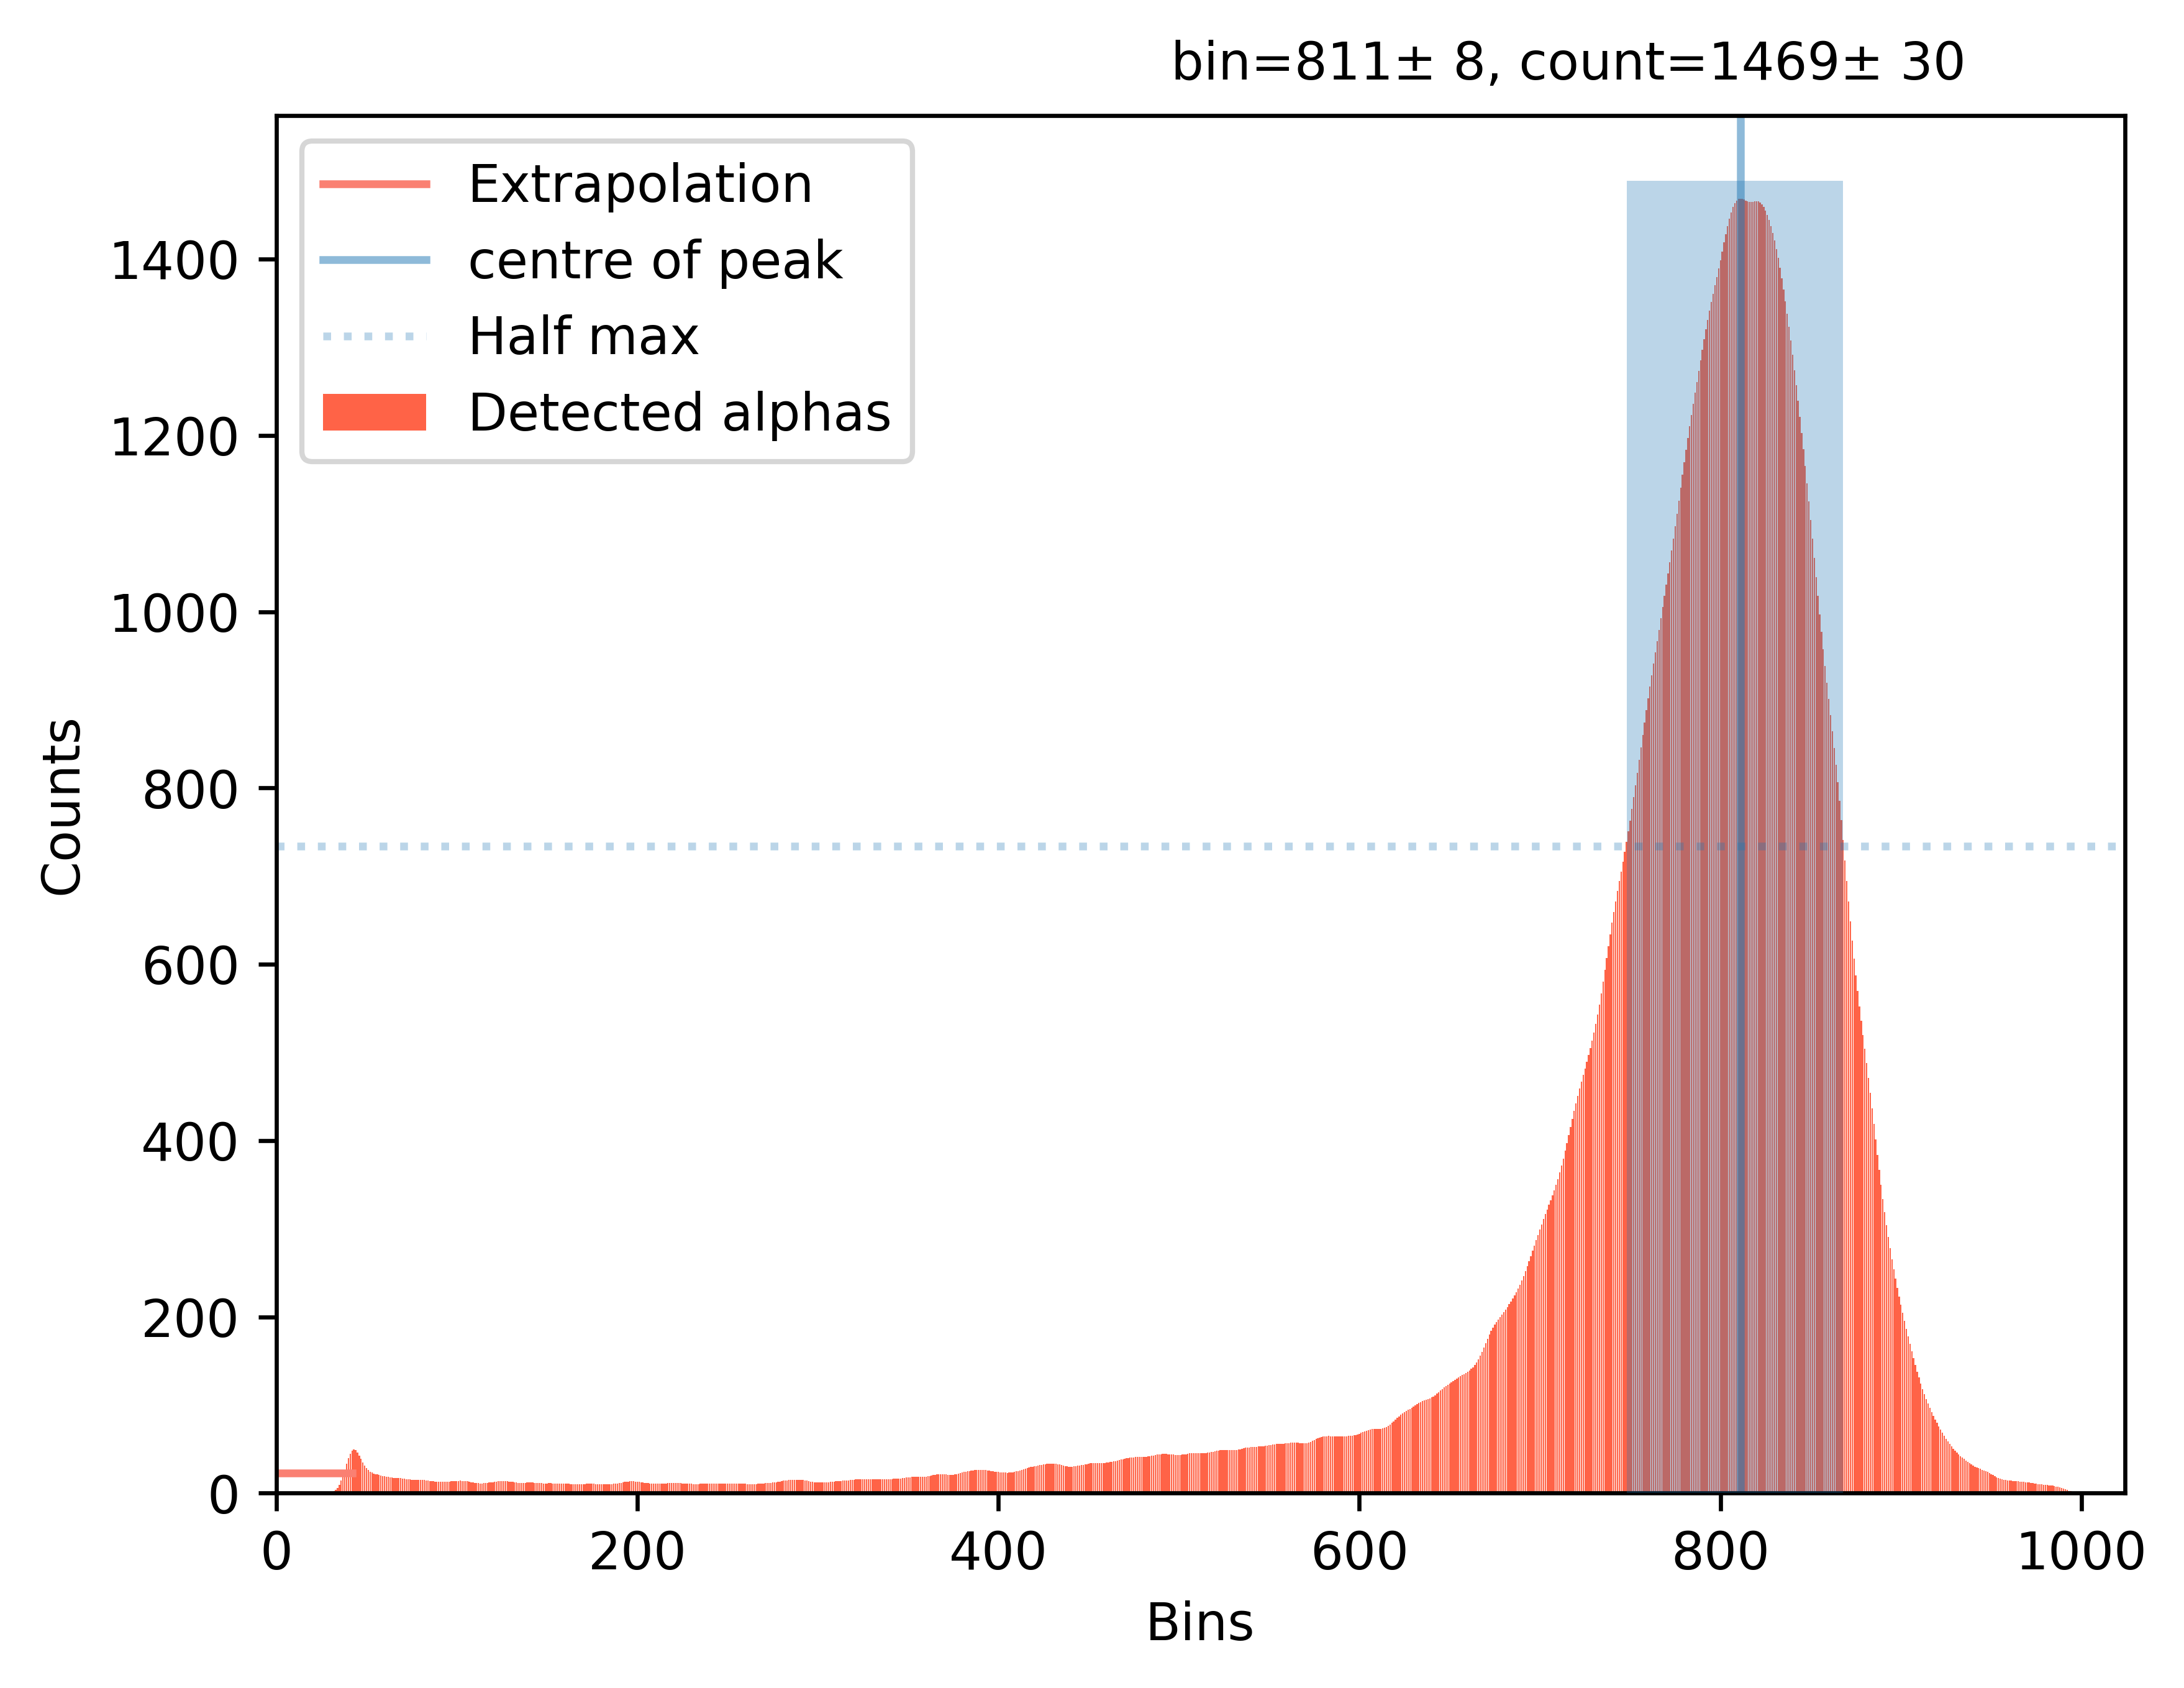
\includegraphics{smooth_p=5.17kPa.png}
}}
\subfloat[]{\scalebox{0.37}{
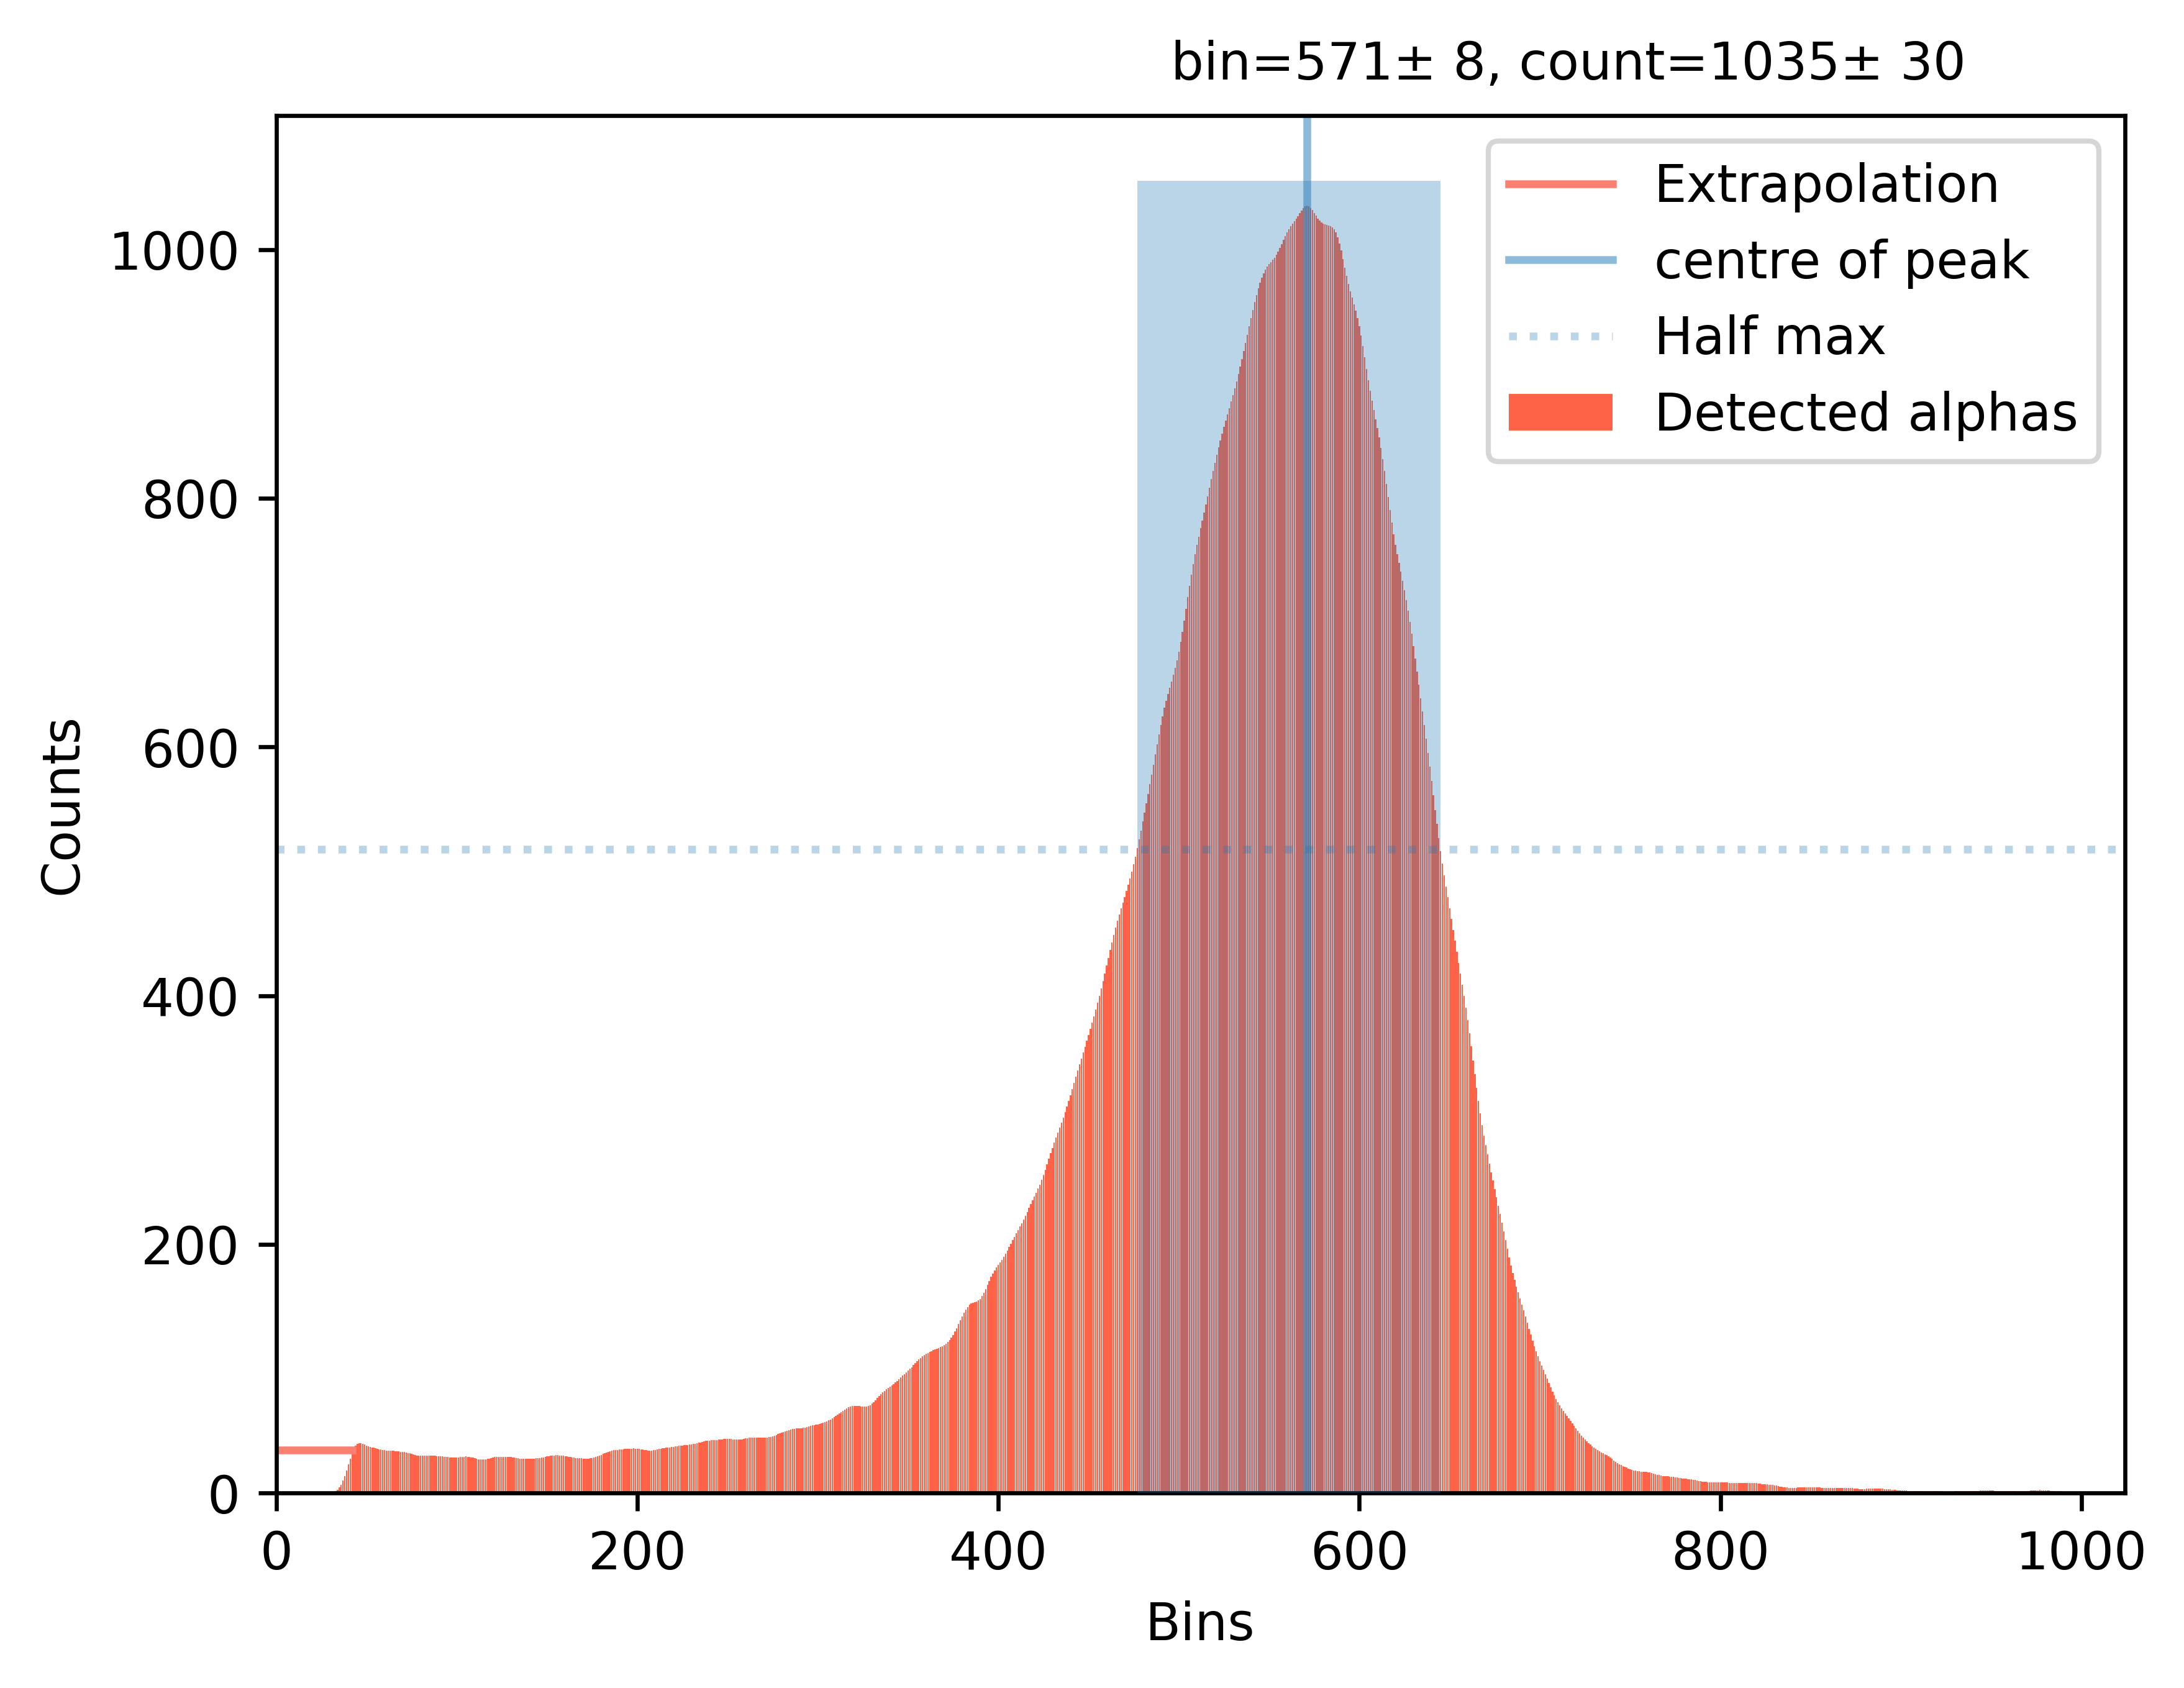
\includegraphics{smooth_p=19.97kPa.png}   
}}
\subfloat[]{\scalebox{0.37}{
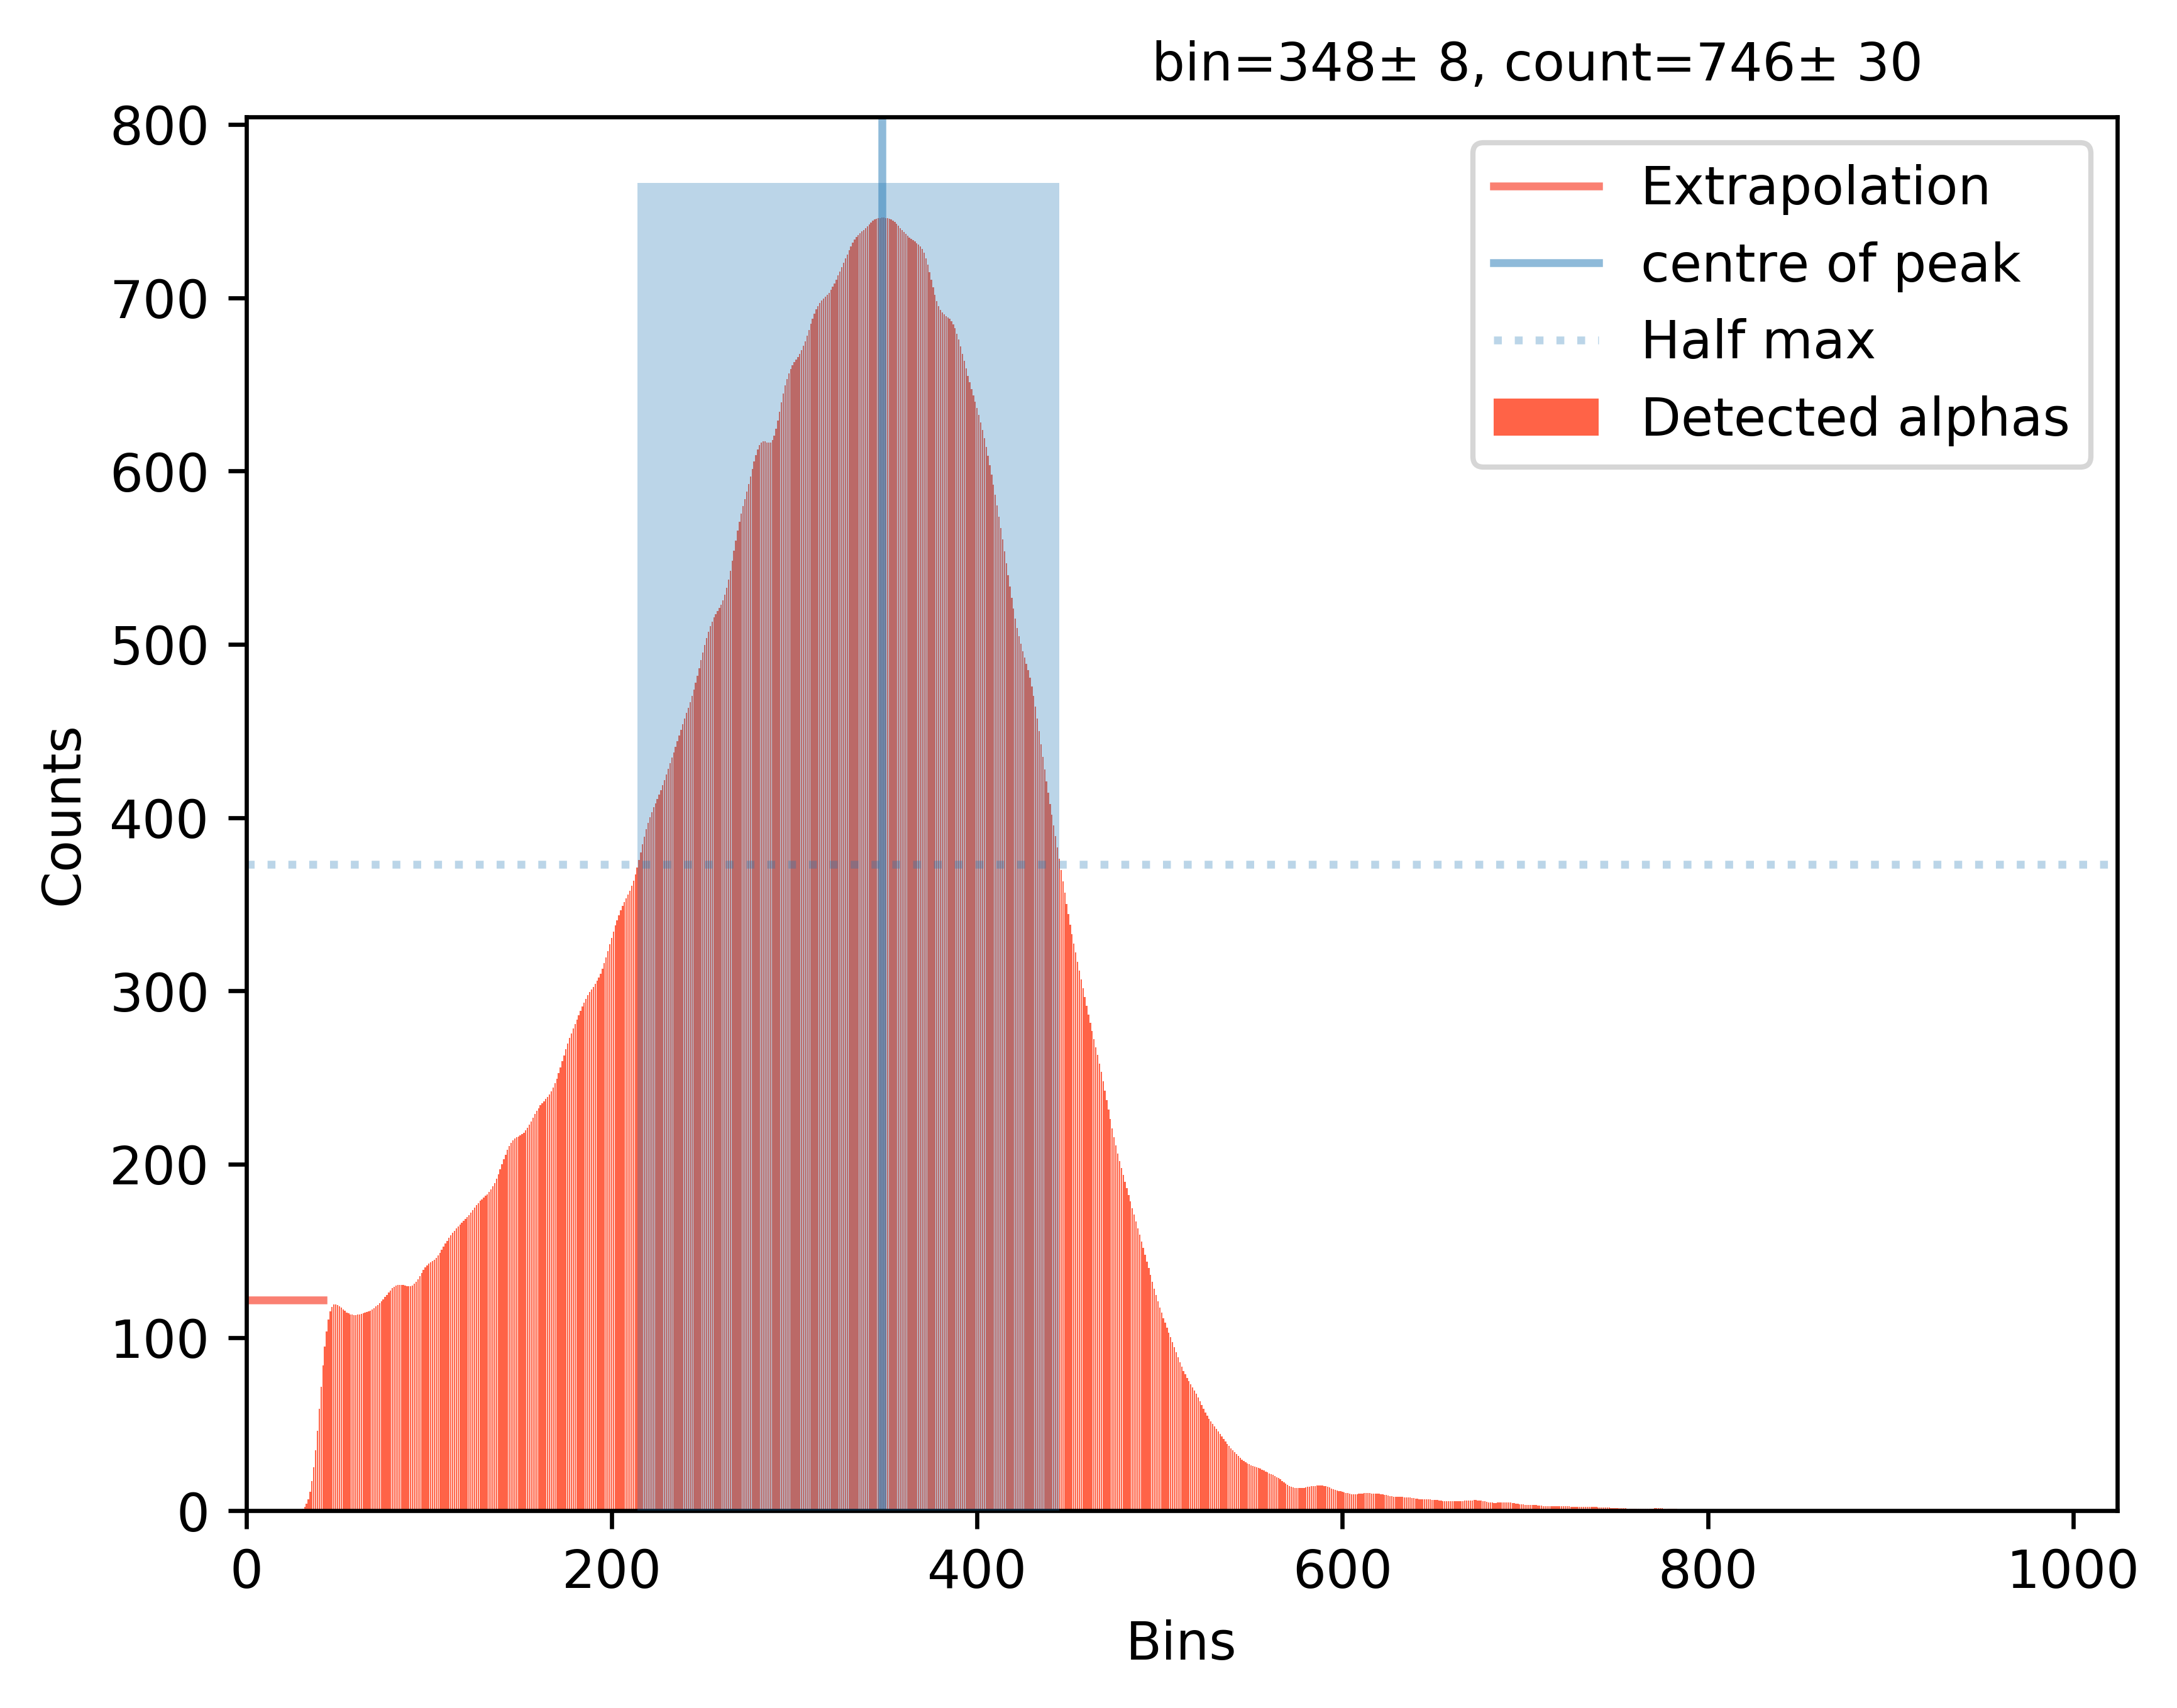
\includegraphics{smooth_p=30.07kPa.png}
}}
\caption{Example of unprocessed and processed spectra for alpha particle range. Spectra (a),(b),(c) are the raw data. Spectra (d),(e),(f) have been processed using gaussian smoothing. from this smoothed data we created a fit for the peak and the FWHM region. In addition to the data in the the smoothed spectra plots, we have included our extrapolation for the region below the noise threshold. It can be observed (from left to right) that as pressure increases the whole spectrum of the detected alpha particles moves towards the low energy region.
All the spectra in this figure diplay the maximum count, and the bin corresponding to this maximum count in the top right corner of each plot
pressure values 5.17 kPa, 19.97 kPa and 30.07 kPa respectively. }
\end{figure}

\begin{SCfigure}
\caption{
 We found the bin location corresponding to zero energy using the background spectrum recorded with a threshold of 4 bins. 
 We fit a gaussian to this spectrum and from our fit we find the zero energy point to be $10.21 \pm 0.04$.
 }
\includegraphics[width=0.5\textwidth]%
    {background.png}%
\end{SCfigure}

\begin{SCfigure}
\subfloat[]{\scalebox{0.6}{
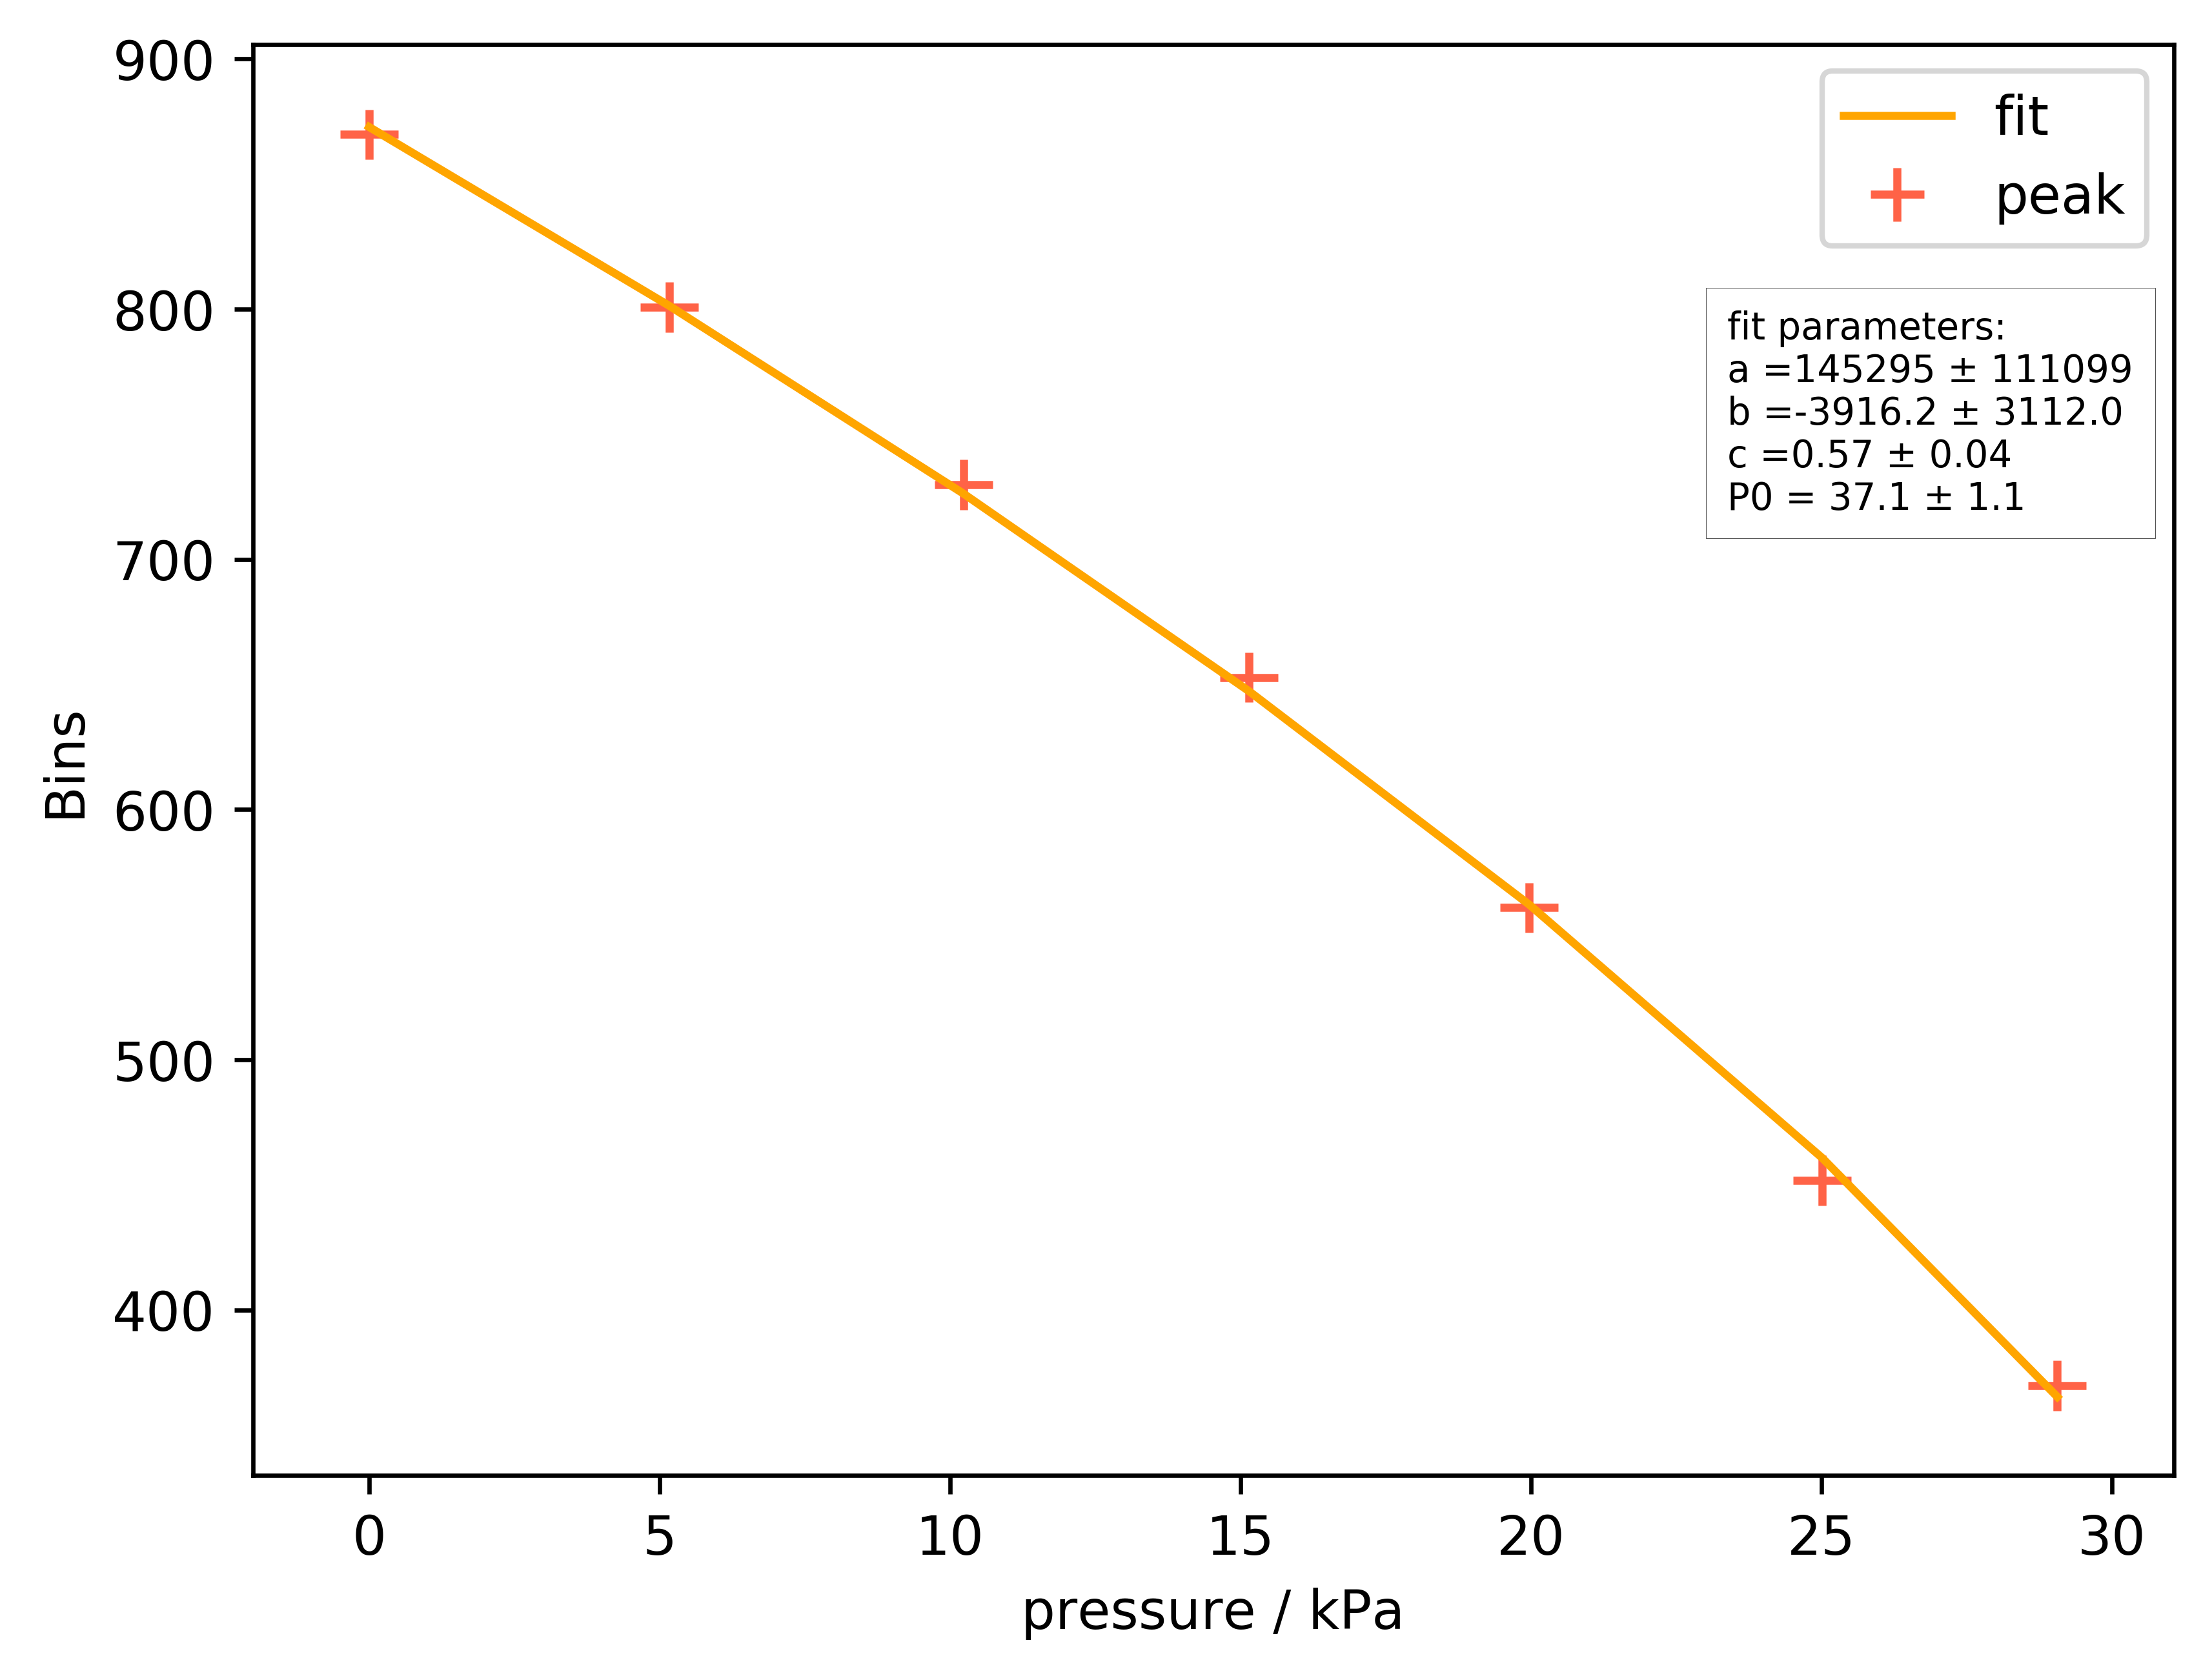
\includegraphics{peak_position_vs_pressure.png}
}}
\caption{
We determined the pressure value $P_0$ corresponding to the absorption of alpha particles with the most probable energy by making a power-law fit of the 6 highest energy (smoothed data) peak values using the equation $y=(a+bp)^c$, where y is peak location, p is pressure. 
Firstly, We subtract the zero energy bin $10.21 \pm 0.04$ from all the peaks positions used in the fit. From our fit we find the pressure value $P_0 = 37 \pm 1$.
The fit parameter values are displayed in the figure. 
}
\end{SCfigure}

\begin{figure}[!htb]
\subfloat[]{\scalebox{0.6}{
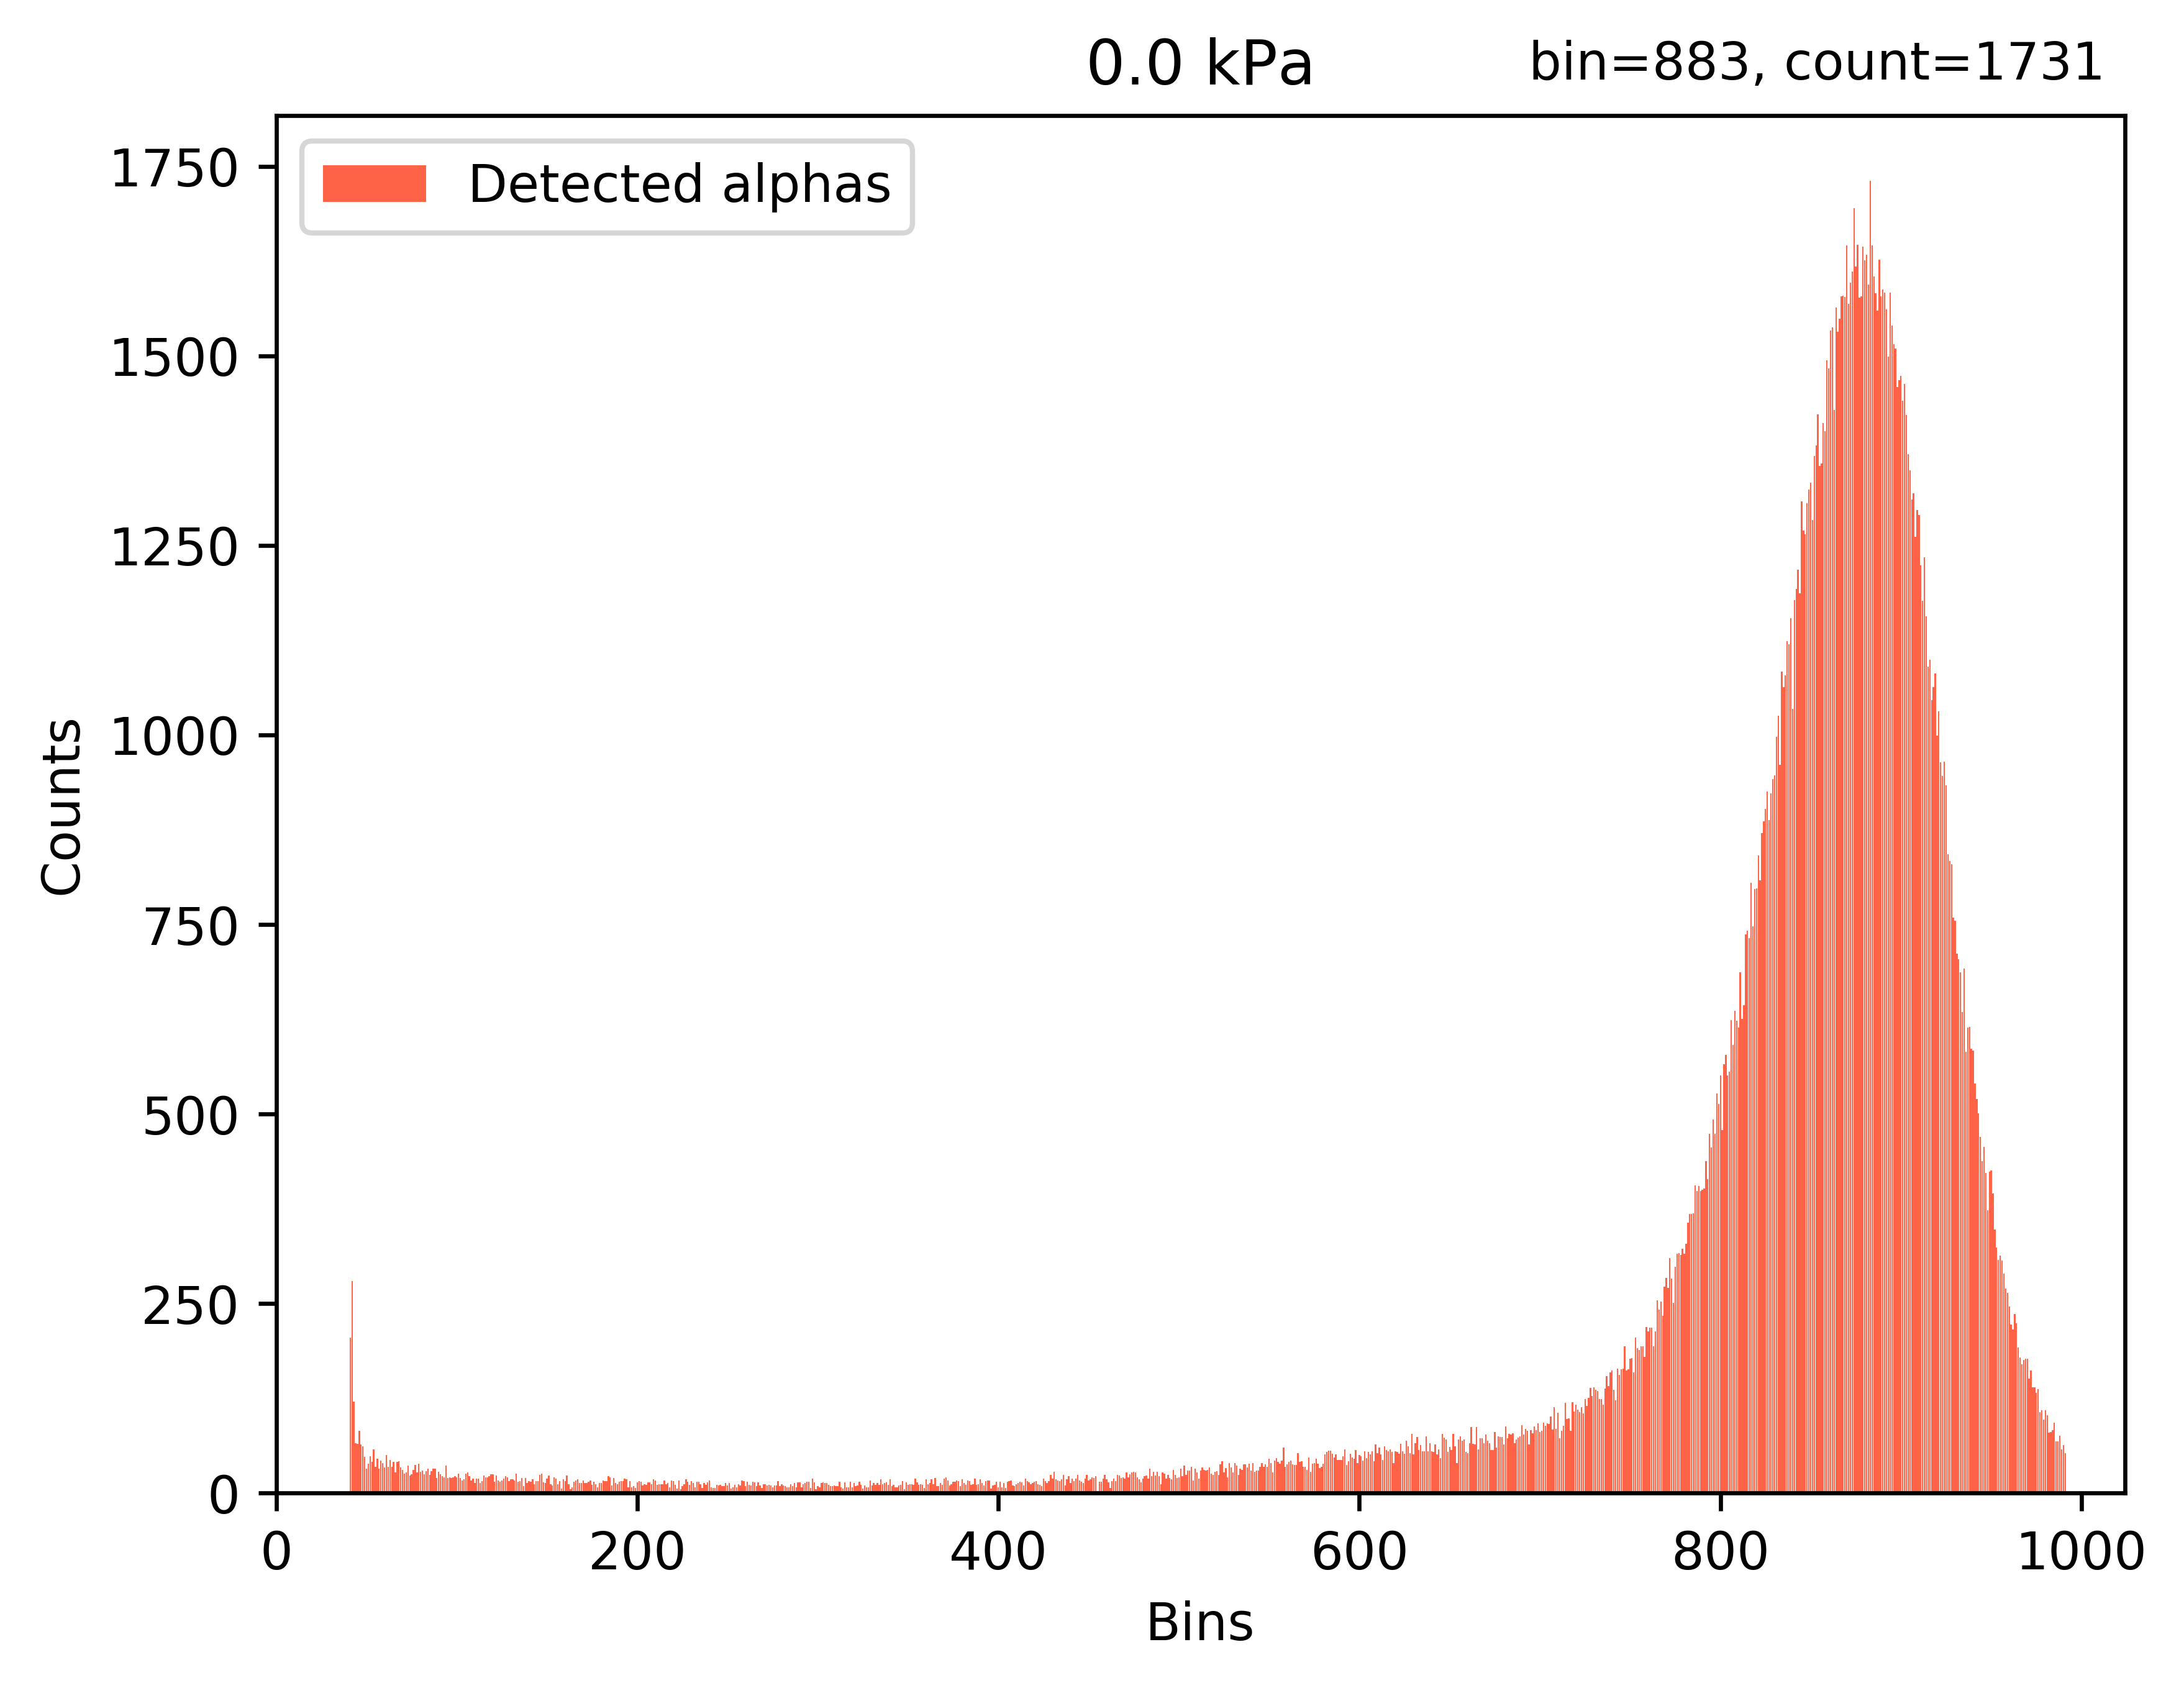
\includegraphics{raw_p=0.0kPa.png}    
}}
\subfloat[]{\scalebox{0.6}{
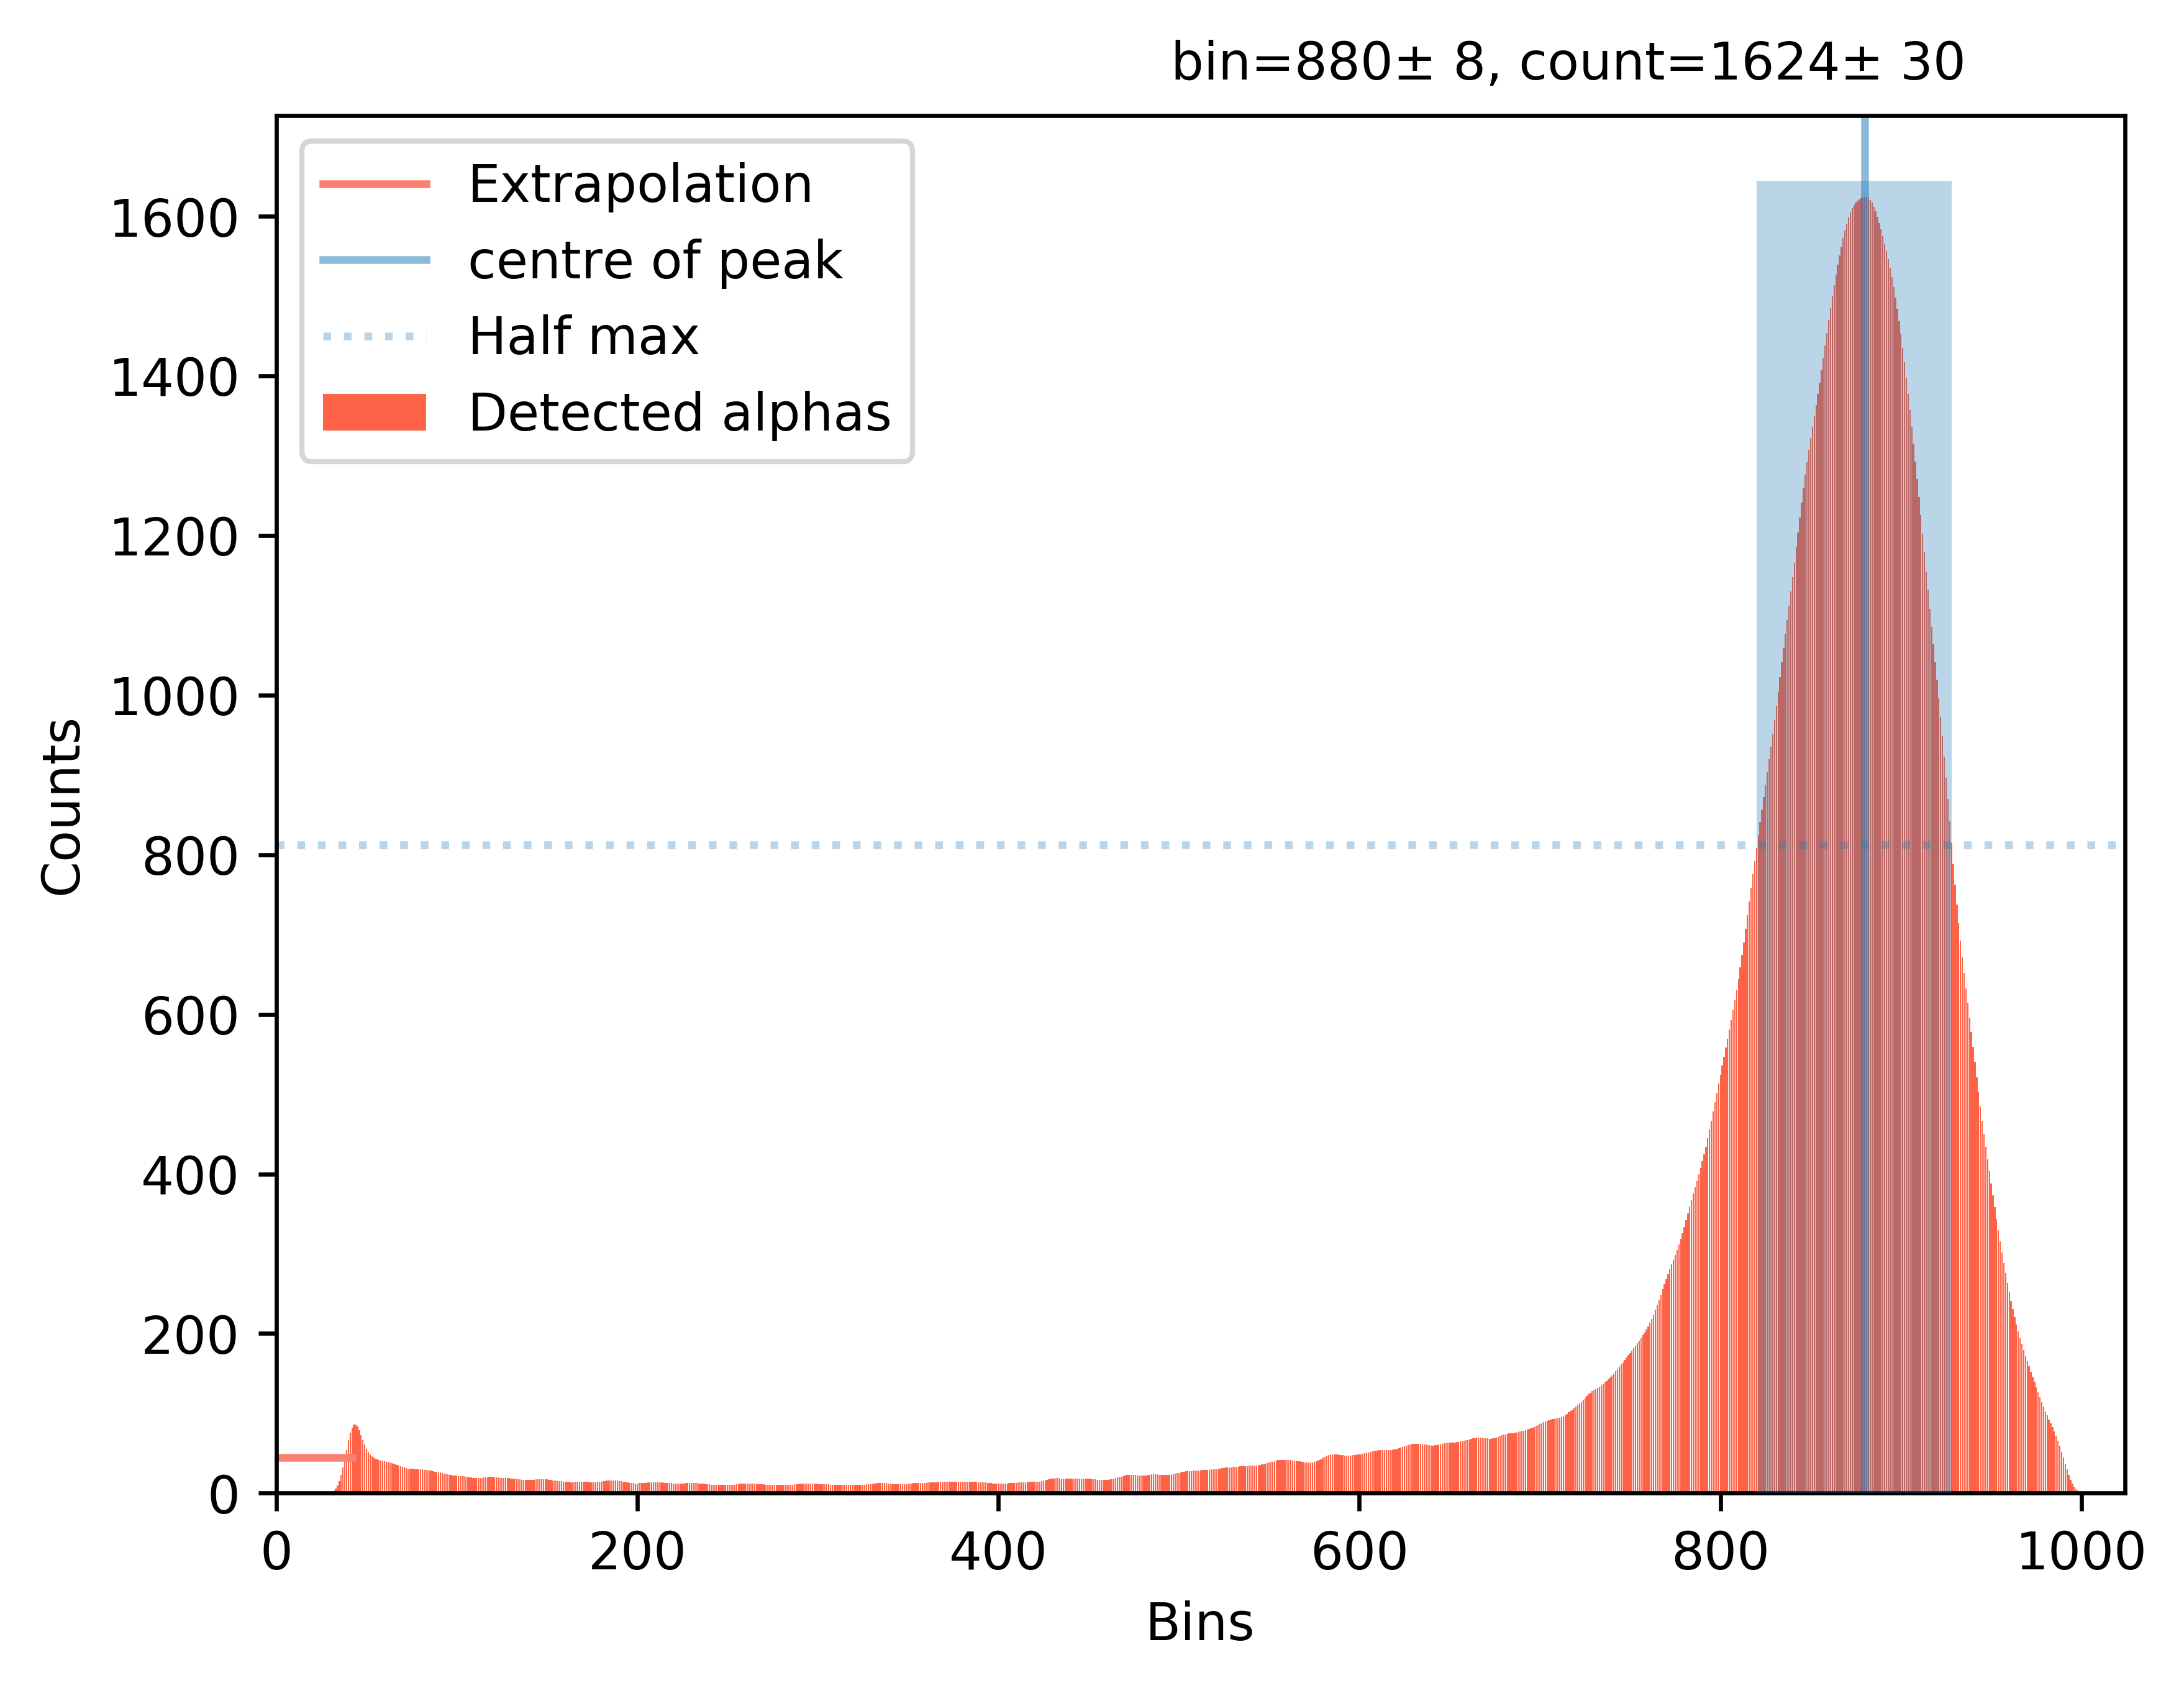
\includegraphics{smooth_p=0.0kPa.png}   
}}
\caption{
Using equation (6), we determine the alpha particle energy (as they are emitted from the source) to be $E_0 = 4.46 \pm 0.09$MeV. We compare the result to the energy emitted from \textsuperscript{241}Am $E = 5.4857$ MeV\cite{SPA}. The difference in these values is $1.03 \pm 0.09$.
To determine the calibration factor for the MCA in terms of the energy, we use the bin corresponding to $E_0$ in the gaussian smoothed distribution in figure (b) and we subtract the zero point energy bin from this and simply calculate the calibration factor $1$bin$ = 5.1 \pm 0.1$keV
}
\end{figure}


\newpage
\begin{multicols}{2}
\section{Discussion}
The width of the energy peaks compared to the energy resolution of the detector requires us to consider the implications of changing the number of bins used. A smaller number of bins gives a higher count in each bin, which improves the signal to noise ratio in each bin because the uncertainty goes as the square root of the number of counts.
A larger number of bins gives a higher resolution of the spectrum, allowing us to find the centre more accurately, but the uncertainty in each bin height becomes bigger by the same reasoning as above.\cite{feedback}
In the case of this experiment most of the spread in our spectra is likely due to the alpha particles travelling through the gold layer that is part of the radioactive source construction. 

In task 1 of our analysis we were unable to determine a way to fit the peaks of our spectra to equation (10). We attempted to make the value of $E_0$ as a fit variable. But we did not manage to obtain a way to convert from bin units to Energy units at this stage.


\section{Conclusion}



\end{multicols}
\bibliography{mybib}
\bibliographystyle{unsrt}
\end{document}


% \begin{equation} 
% \end{equation}


% \begin{equation} ,
% \end{equation}

